% !TEX root = main.tex
%%%%%%%%%%%%%%%%%%%%%%%%%%%%%%%%%%%%%%%%%%%%%%%%%%%%%%%%%%%%%%%%%%%%%%%%%%%%%%%
%  Internship report / Master's thesis
%  Leo Leroy -- MSV (Institut Polytechnique de Paris) & DSSA (ENSAE)
%  Research internship at Nanyang Technological University, Singapore
%
%  Compile with pdflatex (Times is provided by the newtx package).
%  If you prefer to compile with XeLaTeX/LuaLaTeX with the real
%  "Times New Roman" font file, comment out the newtx lines and use:
%     \usepackage{fontspec}
%     \setmainfont{Times New Roman}
%%%%%%%%%%%%%%%%%%%%%%%%%%%%%%%%%%%%%%%%%%%%%%%%%%%%%%%%%%%%%%%%%%%%%%%%%%%%%%%

\documentclass[12pt,a4paper]{article}

%---------------------------------------------------------------- encoding ----
\usepackage[utf8]{inputenc}
\usepackage[T1]{fontenc}
\usepackage[english]{babel}

%------------------------------------------------------------------- maths ----
% (amsmath must be loaded before newtxmath)
\usepackage{amsmath,amsthm,mathtools}

%------------------------------------------------------------------- fonts ----
\usepackage{newtxtext}          % Times New Roman clone for the text
\usepackage[varg]{newtxmath}    % matching mathematics (provides the AMS symbols)
\usepackage{bbm}
\usepackage{bm}

%----------------------------------------------------------------- margins ----
\usepackage[a4paper,
            left=2.4cm, right=2.4cm,
            top=2.6cm, bottom=2.6cm,
            headheight=15pt]{geometry}

%--------------------------------------------------------------- line space ---
\usepackage{setspace}
\onehalfspacing                 % 1.5 line spacing

%--------------------------------------------------------------- graphics -----
\usepackage{graphicx}
\usepackage{subcaption}
\usepackage{booktabs}
\usepackage{array}
\usepackage{multirow}
\usepackage{tikz}
\usetikzlibrary{positioning,arrows.meta,calc}
\usepackage[most]{tcolorbox}
\usepackage{float}


\usepackage{pgfplots}
\pgfplotsset{compat=1.18}      % or newer; without this you'll get warnings
\usetikzlibrary{arrows.meta}   % required for Stealth
\usepackage{xcolor}
\usepackage{caption}

\definecolor{ensae}{HTML}{FF0000}
\definecolor{pure-green}{HTML}{00FF00}
\definecolor{pure-blue}{HTML}{0000FF}

% float placement: avoid half-empty pages around the many figures
\renewcommand{\topfraction}{0.92}
\renewcommand{\bottomfraction}{0.75}
\renewcommand{\textfraction}{0.07}
\renewcommand{\floatpagefraction}{0.80}
\setcounter{topnumber}{3}
\setcounter{bottomnumber}{2}
\setcounter{totalnumber}{5}
\setlength{\parindent}{0pt}
\setlength{\textfloatsep}{12pt plus 2pt minus 3pt}
\setlength{\intextsep}{10pt plus 2pt minus 3pt}
\setlength{\floatsep}{10pt plus 2pt minus 3pt}

%--------------------------------------------------------------- captions -----
\usepackage[font=small,labelfont=bf,margin=0.6cm]{caption}

%----------------------------------------------------------------- layout -----
\usepackage{fancyhdr}
\usepackage{enumitem}
\setlist{itemsep=2pt,topsep=4pt}
\usepackage{titlesec}
\titleformat{\section}{\normalfont\Large\bfseries}{\thesection}{0.8em}{}
\titleformat{\subsection}{\normalfont\large\bfseries}{\thesubsection}{0.8em}{}
\titleformat{\subsubsection}{\normalfont\normalsize\bfseries}{\thesubsubsection}{0.8em}{}

\usepackage[colorlinks=true,
            linkcolor=myblue,
            citecolor=myblue,
            urlcolor=myblue,
            linktocpage=true]{hyperref}

%------------------------------------------------------------------ colours ---
\definecolor{myblue}{RGB}{32,72,120}
\definecolor{lightblue}{RGB}{245,248,252}
\tcbset{
  colback=lightblue,
  colframe=myblue,
  boxrule=0.4pt,
  arc=2mm,
  left=2mm, right=2mm, top=1mm, bottom=1mm
}

%------------------------------------------------------------- environments ---
\theoremstyle{definition}
\newtheorem{definition}{Definition}[section]
\newtheorem{example}[definition]{Example}
\newtheorem{remark}[definition]{Remark}
\theoremstyle{plain}
\newtheorem{proposition}[definition]{Proposition}
\newtheorem{theorem}[definition]{Theorem}
\newtheorem{lemma}[definition]{Lemma}
\newtheorem{corollary}[definition]{Corollary}

%--------------------------------------------------------------- shortcuts ----
\newcommand{\fposs}{f_{\bm{\theta}}}
\newcommand{\R}{\mathbb{R}}
\newcommand{\E}{\mathbb{E}}
\newcommand{\Prob}{\mathbb{P}}
\newcommand{\Pbar}{\bar{{P}}}
\newcommand{\Nposs}{\mathcal{N}^{*}}
\newcommand{\Ga}{\mathrm{Ga}^{*}}
\newcommand{\dd}{\mathrm{d}}
\newcommand{\ind}{\mathbbm{1}}
\newcommand{\Var}{\mathrm{Var}}
\newcommand{\Ttip}{T_{\mathrm{tip}}}
\newcommand{\tnoise}{\tau_{\mathrm{noise}}}
\newcommand{\Estar}{\mathbb{E}^{*}}
\newcommand{\Vstar}{V^{*}}
\DeclareMathOperator*{\argmax}{arg\,max}
\DeclareMathOperator*{\argmin}{arg\,min}

\pagestyle{fancy}
\fancyhf{}
\fancyhead[L]{\small\itshape Decoupling epistemic and aleatoric uncertainties in the prediction of the AMOC collapse}
\fancyhead[R]{\small\thepage}
\renewcommand{\headrulewidth}{0.3pt}

%%%%%%%%%%%%%%%%%%%%%%%%%%%%%%%%%%%%%%%%%%%%%%%%%%%%%%%%%%%%%%%%%%%%%%%%%%%%%%%
\begin{document}
%%%%%%%%%%%%%%%%%%%%%%%%%%%%%%%%%%%%%%%%%%%%%%%%%%%%%%%%%%%%%%%%%%%%%%%%%%%%%%%

%------------------------------------------------------------- title page -----

    

\begin{titlepage}
\centering
\vspace*{0.5cm}

{\large Institut Polytechnique de Paris \& ENSAE Paris}\\[0.3cm]
{\large Nanyang Technological University, Singapore}\\[1.6cm]

\rule{\textwidth}{0.6pt}\\[0.6cm]
{\LARGE\bfseries Decoupling epistemic and aleatoric uncertainties\\[0.35cm]
in the prediction of the AMOC collapse}\\[0.6cm]
{\large A possibilistic revision of the tipping-time estimation\\ of Ditlevsen \& Ditlevsen (2023)}\\[0.5cm]
\rule{\textwidth}{0.6pt}\\[1.4cm]

{\large Research internship report}\\[0.3cm]
{\normalsize Master \emph{Mathématiques pour les Sciences du Vivant} (MSV), Institut Polytechnique de Paris\\
Master \emph{Data Science, Statistique et Apprentissage} (DSSA), ENSAE Paris}\\[1.6cm]

{\Large\bfseries Léo Leroy}\\[1.8cm]

\begin{minipage}{0.46\textwidth}
\raggedright
\textbf{Host supervisor}\\
Prof. Jérémie Houssineau\\
\emph{Nanyang Technological University}\\[0.5cm]
\textbf{Scientific collaborator}\\
Prof. Stéphane Vannitsem\\
\emph{Nanyang Technological University }
\end{minipage}
\hfill
\begin{minipage}{0.46\textwidth}
\raggedleft
\textbf{Academic referees}\\
Prof. Eva Löcherbach\\
\emph{École Polytechnique}\\[0.5cm]
Prof. Matthieu Lerasle\\
\emph{ENSAE Paris}
\end{minipage}

\vfill
{\large Academic year 2025--2026}\\[0.3cm]
{\normalsize \today}
\end{titlepage}




\begin{comment}
    

\begin{titlepage}

% Top Section: Student Info & Institution Info
\noindent
\begin{minipage}[t]{0.48\textwidth}
    \vspace{0pt}
    \textbf{\large LEROY Léo}\\[0.5cm]
    \emph{Academic year 2025--2026}
\end{minipage}
\hfill
\begin{minipage}[t]{0.48\textwidth}
    \vspace{0pt}
    \raggedleft
    \textbf{\large ENSAE 3\textsuperscript{rd} year}\\[0.1cm]
    \textbf{\large Last year internship}
\end{minipage}

\vspace*{6cm}

% Middle Section: Framed Title
\begin{center}
    \fbox{
        \begin{minipage}{0.9\textwidth}
            \centering
            \vspace{1cm}
            {\LARGE\bfseries Decoupling epistemic and aleatoric uncertainties\\[0.35cm]
            in the prediction of the AMOC collapse}\\[0.8cm]
            {\large A possibilistic revision of the tipping-time estimation\\[0.2cm] 
            of Ditlevsen \& Ditlevsen (2023)}\\[1cm]
        \end{minipage}
    }
\end{center}

\vfill

% Bottom Section: Company & Supervisor Info
\noindent
\begin{minipage}[t]{0.48\textwidth}
    \vspace{0pt}
    \raggedright
    \textbf{Nanyang Technological University}\\[0.2cm]
    \textbf{Singapore}
\end{minipage}
\hfill
\begin{minipage}[t]{0.48\textwidth}
    \vspace{0pt}
    \raggedleft
    \textbf{Host supervisor: Prof. J. Houssineau}\\[0.2cm]
    Scientific collaborator: Prof. S. Vannitsem\\
    Academic referees: Prof. E. Löcherbach \& Prof. M. Lerasle\\[0.4cm]
    21/05/2026 to 21/11/2026
\end{minipage}

\end{titlepage}

\end{comment}






%--------------------------------------------------------------- abstract -----


\newpage
\thispagestyle{plain}
\section*{Executive summary}


\noindent
The Atlantic meridional overturning circulation (AMOC) is one of the tipping elements of the
climate system whose collapse would have severe consequences for the North Atlantic region.
The following work is a deepening and improvement of the methodology used by Ditlevsen and Ditlevsen (2023) \cite{ditlevsen2023} to predict the AMOC collapse. They fitted a one-dimensional
stochastic differential equation with a saddle-node bifurcation to a sea surface temperature
fingerprint of the AMOC. By maximum likelihood, they estimated that the critical transition
would occur around 2065, with a $95\%$ confidence interval of $2037$--$2109$. Their statistical
treatment raises three difficulties: the lack of uncertainty propagation, the omission of noise-induced tippings and the lack of uncertainty quantification around the likelihood approximations. \\

\noindent
This report addresses these points using possibility theory in the formulation developed by
J. Houssineau and co-authors. Epistemic uncertainty (due to a lack of knowledge) about deterministic but unknown
parameters is described by possibility functions. It is then combined
with aleatoric uncertainty (due to pure randomness) through Outer Probability Measures. We build a joint possibilistic
posterior over the five parameters of the model with an uninformative prior to represent pure ignorance. The Outer Probability Measure uses a quasi-static approximation of the Eyring--Kramers law to quantify the probability of noise-induced tippings. Simulations show that between
$84\%$ and $90\%$ of the trajectories generated with the estimated parameters tip before the deterministic bifurcation time. We finally display the cumulative credibility and necessity of the tipping time to account for epistemic uncertainty arising in the parameters. \\

\noindent Moreover, we suggest some perspectives. The Eyring--Kramers law used to compute the density of noise-induced tippings is not exact. Solving the Fokker-Planck equation might bring better results. Besides, as the likelihoods used for the estimation are approximation of the likelihood from the true model, they are therefore uncertain. Obtaining bounds to quantify the likelihood deviation or flattening the posterior to artificially increase epistemic uncertainty are two possible ways to deals with this problem. \\

\vspace{0.4cm}
\noindent\textbf{Keywords:} possibility theory, outer probability measures, epistemic uncertainty, stochastic differential equations, saddle-node bifurcation, metastability, Eyring--Kramers law, tipping points, AMOC.



%------------------------------------------------------------------- toc ------
\newpage
\thispagestyle{plain}
{\setstretch{1.15}\tableofcontents}

%-------------------------------------------------------------- notation ------
\newpage
\thispagestyle{plain}
\section*{Notation}

\begin{center}
\renewcommand{\arraystretch}{1.25}
\begin{tabular}{ll}
\toprule
Symbol & Meaning \\
\midrule
$X_t$ & AMOC fingerprint (subpolar gyre SST anomaly), state of the SDE \\
$\theta=(A,m,\lambda_0,\tau_r,\sigma)$ & vector of unknown parameters \\
 $\lambda_t$ & control parameter, $\lambda_t = \lambda_0(1 - \mathbbm{1}(t_0 < t) \frac{t - t_0}{\tau_r})$ \\
$t_0$, $t_c$, $\tau_r$ & start of the ramping ($t_0 = 1924$), bifurcation time, ramping duration \\
$\alpha(\lambda)=2\sqrt{A|\lambda|}$ & local relaxation rate at the stable fixed point \\
$\mu(\lambda)=m+\sqrt{|\lambda|/A}$ & stable fixed point \\
$x_u(\lambda)=m-\sqrt{|\lambda|/A}$ & unstable fixed point \\
$V(x,\lambda)$ & potential, $V(x, \lambda) =A(x-m)^3/3+\lambda(x-m)$ \\
$\Delta(\lambda)$ & potential barrier \\
$\tau_n(\lambda)$ & mean Eyring--Kramers escape time \\
$\Ttip$ & effective tipping time \\
$\fposs$, $f_{\theta\mid x}$ & prior and posterior possibility functions \\
$\Pbar$, $N$ & outer probability measure (credibility), necessity \\
$\omega$ & flattening exponent applied to the posterior \\
\bottomrule
\end{tabular}
\end{center}

\newpage

%%%%%%%%%%%%%%%%%%%%%%%%%%%%%%%%%%%%%%%%%%%%%%%%%%%%%%%%%%%%%%%%%%%%%%%%%%%%%%%
\section{Introduction}
%%%%%%%%%%%%%%%%%%%%%%%%%%%%%%%%%%%%%%%%%%%%%%%%%%%%%%%%%%%%%%%%%%%%%%%%%%%%%%%

The Atlantic Meridional Overturning Circulation belongs to a set of climate
subsystems classified as tipping elements: components of the Earth system that can shift,
largely irreversibly and on a human timescale, from one stable regime to another once a
critical threshold is crossed. Because a collapse of the AMOC would reshape the climate of Western Europe, estimating when such a collapse might occur is a
question with direct societal relevance. Moreover, the uncertainty attached to that estimate matters
as much as the point prediction itself for efficient decision-making. \\
 
\noindent In 2023, Ditlevsen and Ditlevsen published \cite{ditlevsen2023} a statistical of the AMOC collapse. They
reported a $95\%$ confidence interval of $[2037,2109]$ for the year of collapse. Their analysis showed that a collapse can arrive soon, during the current century, unlike former predictions. \\
 
\noindent However, a closer reading of the article's statistical machinery reveals three methodological gaps that are
the object of this report. First, the estimation proceeds in two plugged-in steps, so that the
uncertainty of the first step is silently treated as known when the second step is carried
out. Second, and more consequentially, the quantity that is actually estimated, the deterministic bifurcation time, is not the physically relevant one: the stochastic forcing of
the system can trigger the transition through pure chance well before the bifurcation. Third, the likelihood itself is available only through two successive
approximations, a linearization and a splitting scheme, so that the reported confidence
interval inherits an error whose size is never assessed. \\
 
\noindent This internship was carried out at Nanyang Technological University under the supervision of
Prof. Jérémie Houssineau and the collaboration of Prof. Stéphane Vannitsem. It addresses these three points using possibility theory. This is a statistical framework in
which epistemic uncertainty (due to a lack of knowledge), is represented separately from aleatoric uncertainty (due to pure randomness). Possibility theory helps us model pure ignorance. The plug-in problem, the missing noise-induced tipping, and the approximate
likelihood are three instances of the same underlying question: how much is an inference
entitled to claim once every source of ignorance has been accounted for? \\
 
\noindent The report is organized as follows. Section~\ref{sec:context} introduces the necessary
background: possibility theory and outer probability measures on one hand, the AMOC model and
the original estimation procedure of Ditlevsen and Ditlevsen on the other. Section~\ref{sec:contrib}
develops the contributions of the internship: a joint possibilistic posterior over the five
parameters of the model that removes the plug-in step, and a non-homogeneous escape-rate model
that incorporates noise-induced tipping and shows that it dominates the effective tipping time.
Section~\ref{sec:perspectives} turns to what remains to be done: the technical work needed to
bring the AMOC contribution to a publishable state, and a second  activity undertaken
a few days ago, reviewing a submission for the AAAI conference.  \\


\begin{figure}
    \centering
    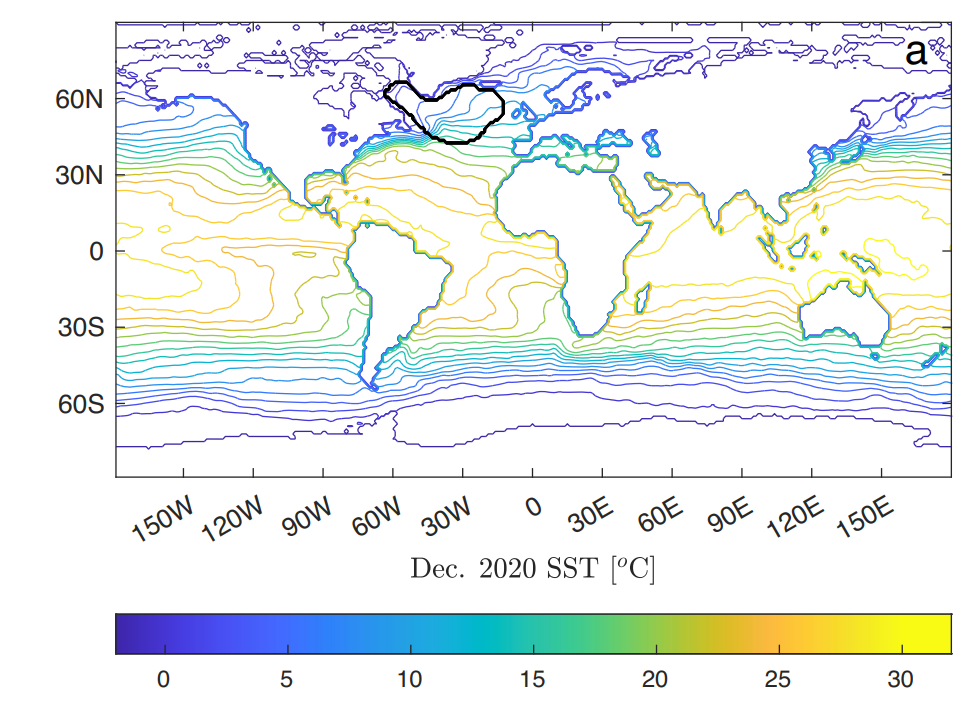
\includegraphics[width=\linewidth]{images/amoc.png}

    \caption{Geographical location of the AMOC (continuous black line) with sea surface temperature (colors) \cite{ditlevsen2023}}
    \label{fig:placeholder}
\end{figure}

\newpage
%%%%%%%%%%%%%%%%%%%%%%%%%%%%%%%%%%%%%%%%%%%%%%%%%%%%%%%%%%%%%%%%%%%%%%%%%%%%%%%
\section{Context}
\label{sec:context}
%%%%%%%%%%%%%%%%%%%%%%%%%%%%%%%%%%%%%%%%%%%%%%%%%%%%%%%%%%%%%%%%%%%%%%%%%%%%%%%


%-------------------------------------------------------------------------------
\subsection{An introduction to possibility theory and epistemic uncertainty}
\label{sec:possibility}
%-------------------------------------------------------------------------------

\subsubsection{Historical context and definitions}

Possibility theory originally stems from fuzzy logic \cite{zadeh1978}. In classical logical, there exists only two truth values: True or False. An element $x$ belongs or does not belong to a set $S$. Fuzzy logic extends classical logic by defining the truth value within $[0,1]$. If $x$ belongs to $S$ with truth value 0.8, it means that "it is mostly true that $x \in S$". This definition of truth has been conceived in order to tackle the inherent uncertainty of linguistic terms in human language. Humans are capable of reasoning with concepts that are ill-defined, namely, with concepts whose definition is fuzzy. The term "small" for example will have different definitions according to different situation. A whale can be perceived as small, while a hen can be perceived as big: both propositions are true within human language. The quantification of such truth values can be made more intelligible when considering Prototype Theory \cite{rosch1973}. A sparrow is a prototypical example of a bird. We can say $ sparrow \in Birds$ with truth value 1. However, a penguin is a bad example of a bird, even though it is still a bird. We could say $penguin \in Birds$ with truth value 0.6. Possibility theory is the mathematical framework that was originally created to be the equivalent of probability theory applied to fuzzy logic. The goal was to obtain rigorous calculation to help reasoning under uncertainties related to fuzzy human concepts. \\


\noindent These concepts help us understand what hides behind the word "uncertainty". Uncertainty quantification is a framework that deals with the characterization and estimation of uncertainties (Wikipedia). As already mentioned in the paragraph above, uncertainty quantification distinguishes aleatoric uncertainty and epistemic uncertainty. Aleatoric uncertainty comes from pure randomness. If we are uncertain about the outcome of a coin toss, it is solely due to its intrinsic randomness. On the other hand, epistemic uncertainty arises when concepts are vague or when we do not have enough data. \\ 


%\begin{widetext}    
        \begin{minipage}{0.5\linewidth}
            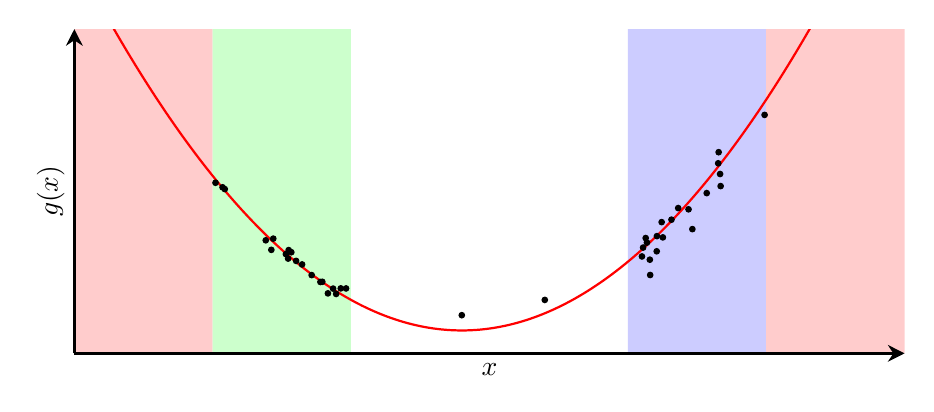
\begin{tikzpicture}
              \begin{axis}[
                width=\linewidth,
                height=5.7cm,
                xmin=-15, xmax=15,
                ymin=0,   ymax=170,       % axe y de 0 à 170
                xlabel={$x$},
                ylabel={$g(x)$},
                axis on top,
                axis lines=left,
                ticks=none,
                axis line style={
                  line width=1pt,
                  -{Stealth[length=6pt,width=6pt]}
                },
                clip=true,               % clip réactivé
              ]
            
                % arrière-plan coloré (y de 0 à 170)
                \addplot [ensae!20,  fill=ensae!20,  draw=none]
                  coordinates {(-15,0) (-15,170) (-10,170) (-10,0)} \closedcycle;
                \addplot [pure-green!20, fill=pure-green!20, draw=none]
                  coordinates {(-10,0) (-10,170)  (-5,170)  (-5,0)}  \closedcycle;
                \addplot [white!20,      fill=white!20,      draw=none]
                  coordinates {(-5,0)   (-5,170)   (5,170)   (5,0)}   \closedcycle;
                \addplot [pure-blue!20,      fill=pure-blue!20,      draw=none]
                  coordinates {(5,0)    (5,170)    (10,170)  (10,0)}  \closedcycle;
                \addplot [ensae!20,  fill=ensae!20,  draw=none]
                  coordinates {(10,0)   (10,170)   (15,170)  (15,0)} \closedcycle;
            
                % fonction vraie g(x)=x^2+2x+3 décalée de +10
                \addplot [domain=-15:15, samples=200, ensae, thick] {x^2 + 2*x + 3 + 10};
            
                % points d'entraînement y+10
                \addplot [only marks, mark=*, black, mark size=1pt] coordinates {
                  % région [-10,-5]
                  (-7.256,54.125) (-6.424,41.010) (-6.986,48.461) (-7.276,49.675)
                  (-7.882,54.252) (-6.771,46.606) (-7.812,60.133) (-5.541,31.138)
                  (-5.182,34.026) (-8.083,59.257) (-6.041,37.507) (-7.356,52.018)
                  (-7.160,53.008) (-5.372,34.053) (-9.645,87.043) (-9.564,86.104)
                  (-9.899,89.415) (-5.837,31.434) (-6.109,37.408) (-5.650,33.935)
                    % center
                    (-1, 20)
                    (2, 28)
                  
                  % région [5,10]
                  (8.334,94.012)  (8.353,87.676)  (6.052,61.448)  (5.645,60.434)
                  (6.577,70.078)  (6.819,76.155)  (7.851,83.997)  (7.193,75.498)
                  (9.942,125.000) (5.510,50.787)  (6.044,53.492)  (5.807,41.066)
                  (8.266,99.625)  (6.266,60.784)  (7.332,65.113)  (6.222,68.787)
                  (5.795,49.097)  (5.552,55.447)  (8.282,105.440) (5.691,58.058)
                };
            
              \end{axis}
            \end{tikzpicture}
            \captionof{figure}{Illustration of aleatoric and epistemic uncertainties for a 1D regression.}
            \label{fig:uncertainty}
        \end{minipage}
        %
        \hfill
        %
        \begin{minipage}{0.5\linewidth}
            %
            \begin{itemize}
                \item In red, epistemic uncertainty is high as there is no training data.
                \item In white, epistemic uncertainty is lower because there are 2 points. 
                \item In green, there are many points with low variance (low epistemic \/ aleatoric uncertainties). 
                \item In blue, aleatoric uncertainty is higher while epistemic uncertainty is low.
            \end{itemize}
        \end{minipage}
    %\end{widetext}




\subsubsection{Decoupling aleatoric and epistemic uncertainty: J. Houssineau's research}

We introduce here the extensions and uses of possibility theory developed by Jérémie Houssineau \cite{ipsa}. \\

\noindent With possibility theory, we can define a new object in a similar manner as we define random variables. The goal is to describe the information or uncertainty about a fixed parameter $\theta^* \in \Theta$ that we want to estimate. Let $\Omega_u$ be the states of nature. Among them, $\omega^*$ is the \emph{true} state of nature. We define a \emph{deterministic uncertain variable} $\bm{\theta} : \Omega_u \to \Theta$ such that $\bm{\theta}(\omega^*) = \theta^*$. The information about $\theta^*$ is describe by a possibility function $f_{\bm{\theta}} : \Theta \to [0,1]$ verifying $\sup\limits_{\theta \in \Theta} f_{\bm{\theta}}(\theta) = 1$. When $\fposs(\theta) = 1$ for all $\theta \in \Theta$, we model \emph{complete ignorance}: all values of $\theta$ are possible. A very important distinction from probability theory is that we cannot sample from possibility function, as they do not describe random events. Moreover, possibility functions are not unique: a deterministic uncertain variable accepts many possibility functions, depending on how observers define the information about $\theta$. If $\fposs$ describe $\bm{\theta}$, then any $g \geq \fposs $ pointwise also describes $\theta$, but with less information. This highlights the subjective nature of epistemic uncertainty. \\ 

\noindent From the possibility function, we can define an \emph{Outer Probability Measure} (OPM) as $\bar{P}(A) := \sup\limits_{\theta \in A} \fposs(\theta)$, $A \subset \Theta$. When $\bar{P}(A) = 1$, there is no evidence against $\theta^* \in A$. The OPM has the same properties as a probability measure, except that for two disjoint sets $A$ and $B$, $\bar{P}(A \cup B) = \max(\bar{P}(A), \bar{P}(B))$ instead of $\bar{P}(A) + \bar{P}(B)$. We fall back on the definition of a probability if we replace the possibility function $\fposs$ by a density $p$ and the $\sup$ operator by an integral. \\

\noindent We can recover the equivalent of Bayes rule: for data $X$, likelihood $L$ and a prior $\fposs$, we get that the posterior verifies:
$$
f_{\bm{\theta} \mid X }(\theta \mid X) = \frac{L(X \mid \theta) \cdot \fposs(\theta)}{\sup_{\psi \in \Theta}L(X \mid \psi) \cdot \fposs(\psi)}
$$

\noindent Notice that this form of posterior closely resembles the probabilistic Bayes theorem, where the integral has been replaced by a supremum. This implies that if we use the uninformative prior $\fposs(\theta) = 1$, the posterior is still perfectly defined, while the integral would diverge. This enables to start from a uninformative prior for any statistical problem, while the definitions of uninformative priors in the probabilistic Bayesian settings can sometimes be complex. Moreover, if we use this uninformative possibilistic prior, we obtain a relative likelihood ratio: the posterior becomes the likelihood divided by the maximum of likelihood. \\

\noindent Finally, we can combine probability and possibility to decouple aleatoric and epistemic uncertainty. An \emph{uncertain variable} is a mapping $\mathcal{X} : \Omega_u \times \Omega_r \to S$, with $(\Omega_r, \mathcal{E}, \Prob(\cdot \mid \omega_u))$ a probability space. For a deterministic uncertain variable $\bm{\theta}$ described by $\fposs$ and $Y \mid \bm{\theta}$ described by the probability distribution $p(\cdot \mid \bm{\theta})$, we get that the uncertain variable $\mathcal{X}$ with uninformative prior can be described by the OPM:
$$
\bar{P}(A) = \sup_{\theta \in \Theta} f(\theta \mid X)  \cdot \int_A p(y \mid \theta) dy
$$

\noindent This OPM also defines the \emph{necessity function} as $N(A) := 1 - \bar{P}(A^c)$. We therefore get that for all events $A$, the probability of $A$ is in the interval $[N(A), \bar{P}(A)]$. The tighter this interval, the lower the epistemic uncertainty. The interpretation is as follows: $\Pbar$ is the largest probability that can be produced by a parameter value which the data do not contradict. 




\subsubsection{Why probability theory is not enough}

\noindent The reason why probability cannot correctly account for epistemic uncertainty is \emph{additivity}. Among the axioms of probability theory, we have that for an event $A \in \Omega$, $P(A) + P(A^c)$ = 1, where $A^c$ is the complement of $A$. This axiom is very natural for random events, but it does not work with epistemic uncertainty. When ignorance is complete about an event $A$, we cannot know if $A$ or $A^c$ is likely. Assigning a value to $P(A)$ automatically assigns the value $1 - P(A)$ for $P(A^c)$. \\

\noindent With possibility theory, if the ignorance is complete about $A$, we can say "$A$ is possible and so is $A^c$". This translates into $\bar{P}(A) = \bar{P}(A^c) = 1$, where $\bar{P}$ is called a credibility function. A credibility of 1 means that the event is completely possible, or equivalently that there is no proof against this event. The operator that allows such equality is the $\max$ operator (or $\sup$ if we work on non compact sets). \\


\noindent Another reason why we should avoid an additive operator (like the sum or the integral) is probability dilution. When a satellite needs to dodge orbital debris, the debris's exact path is unknown. Paradoxically, if we use standard probability to model this, having worse data actually makes the calculated risk of collision lower. If $\sigma$ is the variance (uncertainty) of the debris's location, a greater $\sigma$ means a greater uncertainty. If the debris's location follows a normal distribution, a greater $\sigma$ implies a flatter bell curve. As the mode decreases, the probability concentrated inside a small collision zone drops to 0. The fact that the area under the bell curve must be preserved to 1 dilutes the probability. As the $\sup$ operator is local, the spread of $f_\theta$ outside $A$ does not change the credibility of $A$. The $\sup$ operator enables to answer the question "what is the most possible scenario in this zone?" and can keep the estimated risk high instead of diluting it. \\





%-------------------------------------------------------------------------------
\subsection{The Atlantic meridional overturning circulation}
\label{sec:amoc}
%-------------------------------------------------------------------------------

\subsubsection{Definitions and data}

\noindent The Atlantic Meridional Overturning Circulation (AMOC) \cite{ditlevsen2023} is the main ocean current system in the Atlantic Ocean and a major component of Earth's climate system. It functions as a continuous global conveyor belt, featuring a northward flow of warm, salty water in its upper layers and a southward return flow of cold, deep water. Warm water from the south is more saline, and as it reaches the north and cools down, its density increases, causing it to sink into the deep ocean. This sinking process transfers heat toward the northern hemisphere. This keeps regions like Northern Europe significantly warmer than they would otherwise be, especially compared to North Eastern American cities like New York at the same latitudes. \\

\noindent A forthcoming collapse of the AMOC is a major concern because it is an important tipping element in the Earth's climate system. If the tipping point is reached, European climate would be durably impacted and it would affect its inhabitants. In climate science, a tipping point is a critical threshold that, when crossed, leads to large, accelerating, and often irreversible changes in the climate system. When a system goes past this point, it undergoes an abrupt, self-propelling shift into an alternative stable state, meaning it does not return to its initial condition even if the drivers of the change are abated. \\

\noindent According to Ditlevsen \& Ditlevsen (2023) \cite{ditlevsen2023}, the AMOC stability is threatened by a changing control parameter like the flux of freshwater into the Northern Atlantic from glacial runoff and ice melt. When this complex system is pushed past a critical value, a structural change in its dynamics happens, forcing the AMOC to bifurcate and move from a previously stable state to a completely different one. \\

%maybe write better this paragraph + PHOTO FROM ARTICLE !!!
\noindent The AMOC collapse is not a matter of consensus withing the scientific community. The AMOC has been continuously measured since 2004 and a decline has been identified, though there is not enough data to conclude about the significance of this decline. According to the  Climate Model Intercomparison Project (CMIP), a collapse of the AMOC is unlikely within the 21st century.  Ditlevsen \& Ditlevsen (2023) \cite{ditlevsen2023} research contradicts this claim and estimates that the tipping could occur between 2037 and 2109 (95\% confidence interval). Because the measured data of the AMOC is too recent to draw conclusions from, they used a fingerprint of the AMOC (see \ref{fig:amoc_ts}): the sea surface temperature in the Sub-polar gyre region of the North Atlantic. These temperatures have been recorded from 1870 to 2020. \\


\begin{figure}
    \centering
    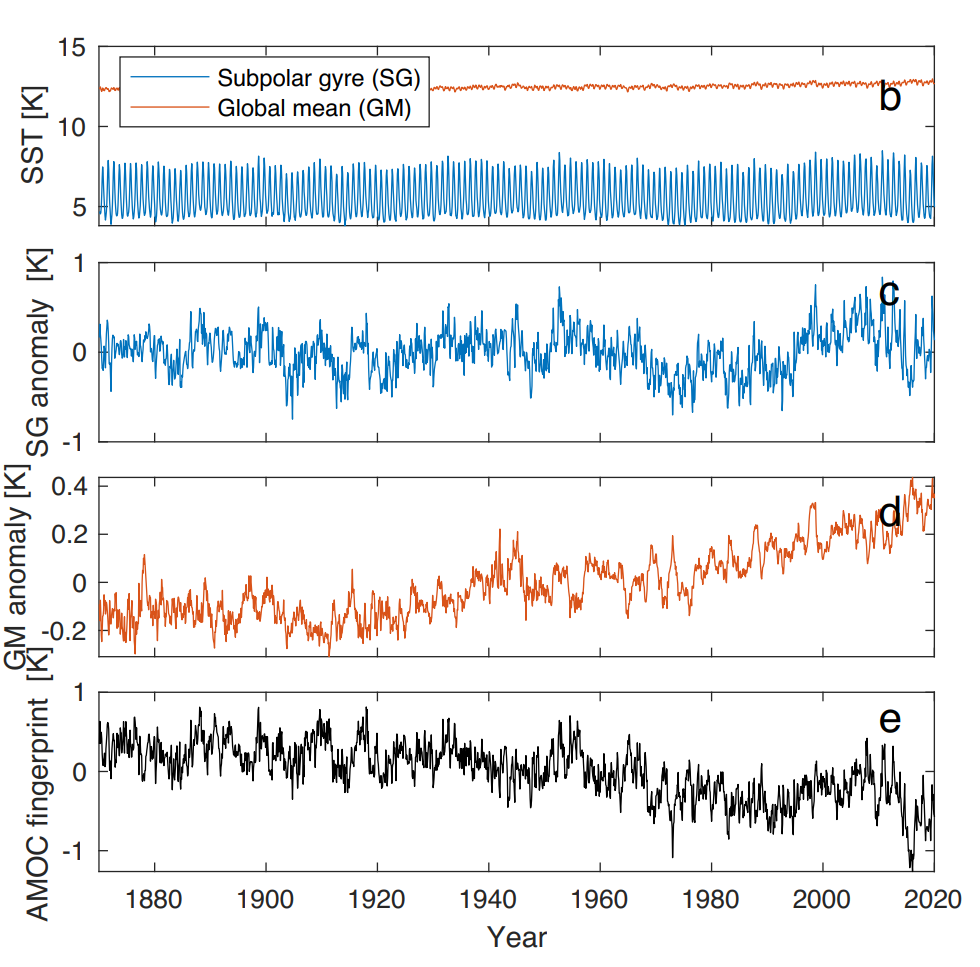
\includegraphics[width=\linewidth]{images/amoc_ts.png}
    \caption{Illustration of the global warming  means (GM) and AMOC fingerprint. In black, the pre-processed data used for the statistical estimation.}
    \label{fig:amoc_ts}
\end{figure}





\subsubsection{Tipping estimation by Ditlevsen \& Ditlevsen (2023) \cite{ditlevsen2023}}


Before estimating the tipping point, they performed two pre-processing steps to the AMOC fingerprint:
\begin{enumerate}
    \item Seasonal cycle removal: because monthly fluctuations in sea surface temperature are driven by solar radiation rather than ocean circulation, they are filtered out by calculating monthly anomalies (subtracting each month's historical long-term average). 
    \item Global warming trend removal: global warming participates in the increase of sea surface temperature, which is not directly related to water circulation changes. They removed twice the global mean SST anomaly. The subtracted this quantity twice because global warming has a stronger effect due to polar amplification. \\
\end{enumerate}

\noindent The AMOC fingerprint is modeled by a stochastic differential equation:
\begin{equation}
\label{eq:model}
\begin{cases}
\dd X_t=-\big(A(X_t-m)^2+\lambda_t\big)\dd t+\sigma\,\dd W_t, \\[4pt]
\lambda_t=\lambda_0\Big(1-\ind(t\ge t_0)\dfrac{t-t_0}{\tau_r}\Big),
\end{cases}
\end{equation}

\noindent with unknown parameter vector $\theta=(A,m,\lambda_0,\tau_r,\sigma)$. They assume that  data was in a stationary state before $t_0$, that they estimated to be equal to 1924. After $t_0$, the fingerprint data become non-stationary and is supposed to represent the observed decline in the real AMOC measurements started in 2004. $\lambda_t$ is a the control parameter, for example fresh water input, assumed to evolve linearly in time. $A$ is a scale parameter. $W_t$ is a Brownian motion of standard deviation $\sigma$. $m = \mu - \sqrt{|\lambda|/A}$ is the stable fixed point of the drift, where $\mu$ is the mean of the process $(X_t)_t$ and $\lambda$ is a value of $\lambda_t$. $\tau_r$ is the ramping time, the time to wait before the system reaches the bifurcation (details below). $t_c = t_0 + \tau_r$ is the (deterministic) tipping time, such that $\lambda(t_c) = 0$. \\

\noindent With the evolving control parameter $\lambda_t$, the system has a \emph{saddle-node bifurcation}. We can rewrite the stochastic differential equation as $dX_t = - \nabla V(X_t)dt + \sigma dW_t$, where $V(x)=A(x-m)^3/3+\lambda(x-m)$ is the potential of the system. This potential has two fixed points. $\mu(\lambda)=m+\sqrt{|\lambda|/A}$ is the stable fixed point and $x_u(\lambda)=m-\sqrt{|\lambda|/A}$ is the unstable fixed point. More figuratively, the potential $V$ defines a landscape in time in which $\mu(\lambda_t)$ is a valley and $x_u(\lambda_t)$ is a mountain. This two fixed points merge at $t=t_c$ (saddle-node bifurcation). \\

\noindent To estimate the parameters, they performed Maximum Likelihood Estimation. To construct confidence intervals, they use Monte Carlo estimation by sampling multiple trajectories from the fitted parameters calculated by MLE (see \ref{fig:simulations_curves}). This is how they obtain that $t_c \in [2037, 2109]$ (95\% confidence interval, see \ref{fig:article_results}). \\







\begin{figure}[htbp]
\centering
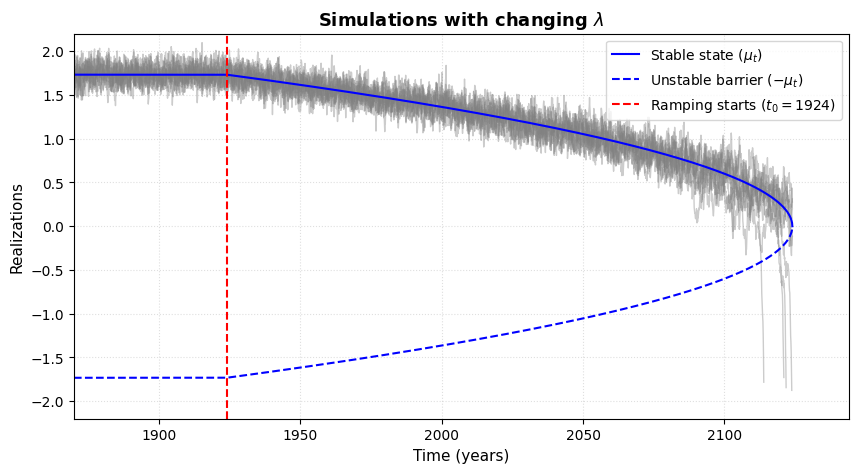
\includegraphics[width=\textwidth]{images/simulations_curves.png}
\caption{Trajectories simulated from model \eqref{eq:model} with the parameters fitted on the
AMOC fingerprint. The stable branch $\mu(\lambda_t)$ decreases and flattens as $t\to t_c$,
while the fluctuations around it grow: this is the joint signature of critical slowing down
and loss of resilience.}
\label{fig:simulations_curves}
\end{figure}

\begin{figure}[htbp]
\centering
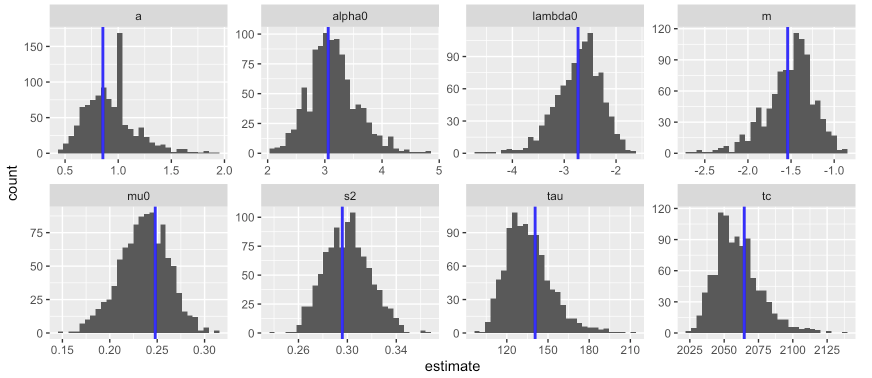
\includegraphics[width=\textwidth]{images/article_results.png}
\caption{Monte Carlo reproduction of the estimation of \cite{ditlevsen2023} on trajectories
simulated with the parameters fitted on the real data. The dispersion of the estimated
bifurcation year is the source of the $95\%$ interval $[2037,2109]$ reported in the article.}
\label{fig:article_results}
\end{figure}

\newpage
%%%%%%%%%%%%%%%%%%%%%%%%%%%%%%%%%%%%%%%%%%%%%%%%%%%%%%%%%%%%%%%%%%%%%%%%%%%%%%%
\section{Contributions on AMOC collapse with Possibility Theory}
\label{sec:contrib}
%%%%%%%%%%%%%%%%%%%%%%%%%%%%%%%%%%%%%%%%%%%%%%%%%%%%%%%%%%%%%%%%%%%%%%%%%%%%%%%


\subsection{Identifying the methodological gaps of the article}

\label{sec:id_AMOC} % DOES NOT WORK !!!!!§§§§§§§§§§§§§§§§§§§§§§§§§§§§§§§§§§

Except the absence of epistemic uncertainty modeling, we saw 2 methodological gaps in the article: 
\begin{enumerate}
    \item The plug-in estimation does not propagate uncertainty correctly.
    \item Noise-induced tippings, that could precipitate the collapse of AMOC, are not studied. \\
\end{enumerate}


\subsubsection{Two-step estimation procedure with plug-in}

Since \eqref{eq:model} has no explicit transition density, the authors proceed in two steps. \\

\noindent \emph{Step 1, stationary regime ($t<t_0$).} With $\lambda_t = \lambda_0$ fixed, and provided
the noise is small enough for the process to stay near the stable point, a Taylor expansion of
the drift around $\mu(\lambda_0)$ gives the linear approximation
\begin{equation}
\label{eq:ou}
\dd X_t\approx-\alpha_0\big(X_t-\mu_0\big)\dd t+\sigma\,\dd W_t,
\qquad \alpha_0=2\sqrt{A|\lambda_0|},\quad \mu_0=m+\sqrt{|\lambda_0|/A} .
\end{equation}
This is an Ornstein--Uhlenbeck process, for which the transition density is Gaussian and exact
maximum likelihood estimators of $(\mu_0,\alpha_0,\sigma)$ are available in closed form
through the stationary mean, the stationary variance $\gamma^2=\sigma^2/(2\alpha_0)$ and the
lag-one autocorrelation $\rho=e^{-\alpha_0\Delta t}$:
\begin{equation}
\label{eq:ou_est}
\hat\alpha_0=-\frac{\log\hat\rho}{\Delta t},\qquad \hat\sigma^2=2\hat\alpha_0\hat\gamma^2 .
\end{equation}
Only two of the five parameters are recovered at this stage, because
\eqref{eq:ou} identifies the combinations
\begin{equation}
\label{eq:link}
\lambda_0(A)=-\frac{\alpha_0^2}{4A},\qquad m(A)=\mu_0-\frac{\alpha_0}{2A},
\end{equation}
leaving $A$ and $\tau_r$ undetermined. These two parameters are \emph{non-identifiable} on stationary data. \\ 

\noindent Notice that we can therefore \emph{equivalently} work with $\theta = (\alpha_0, \mu_0, \sigma, \tau_r, A)$ because the relationship between $\alpha_0$, $\lambda_0$, $m$ and $\mu_0$ are unambiguous. \\

\noindent \emph{Step 2, non-stationary regime ($t>t_0$).} The linear approximation is no longer valid as
the system approaches the bifurcation, and the transition density is unknown. The authors
approximate it by a \emph{Strang splitting} scheme, which is used to separate the deterministic non-linear part of the drift and the stochastic (linearized) part:
\[
\begin{cases}
\dd X^{(1)}_t=-\alpha(\lambda)\big(X^{(1)}_t-\mu(\lambda)\big)\dd t+\sigma\,\dd W_t,\\
\dd X^{(2)}_t=-A\big(X^{(2)}_t-\mu(\lambda)\big)^2\dd t,
\end{cases}
\]
each of which is solvable in closed form, and composes the flows symmetrically as
$\phi^{(2)}_{h/2}\circ\phi^{(1)}_{h}\circ\phi^{(2)}_{h/2}$. Since the resulting transition kernel is a smooth non-linear
transformation of a Gaussian, an explicit likelihood in $(A,\tau_r)$ is obtained. Throughout the rest of this text, we will call this likelihood the "\emph{pseudo-likelihood}". \\

\begin{tcolorbox}
\center \textbf{Methodological gap:} This second-stage likelihood is implicitly conditioned on the
first-stage estimates $(\hat\alpha_0,\hat\mu_0,\hat\sigma)$. The uncertainty of those
estimates is not propagated: the plug-in is treated as exact. \\
\end{tcolorbox}

\noindent Once $(\hat A,\hat\tau_r)$ are obtained, the remaining parameters are recovered through
\eqref{eq:link}, $\hat\lambda_0=-\hat\alpha_0^2/(4\hat A)$,
$\hat m=\hat\mu_0-\hat\alpha_0/(2\hat A)$. As mentioned above, confidence
intervals are then obtained by a parametric bootstrap: $1000$ trajectories are simulated from
\eqref{eq:model} with the estimated parameters and the whole estimation procedure is repeated
on each. \\

\noindent Finally, they get: 
$\hat\alpha_0=3.06$, $\hat\mu_0=0.25$, $\hat\sigma=0.55$, $\hat\tau_r=140.6$, $\hat A=0.86$,
$\hat m=-1.54$, $\hat\lambda_0=-2.73$, and hence $\hat t_c = 2064.6$ (95\% bootstrap confidence interval [2037,\,2109]). \\


\subsubsection{The missing noise-induced tippings}

\paragraph{The results, and the formula that is never used.}


Tipping can occur when a system reaches a bifurcation point, or it can be driven by stochastic perturbations, a phenomenon known as noise-induced tipping. This occurs when the potential barrier, defined by the difference between the stable and unstable states, becomes sufficiently small that random fluctuations can displace the system across the barrier into an alternative state. Here, the potential barrier is equal to: 
\begin{equation}
\label{eq:barrier}
\Delta(\lambda)=V\big(x_u(\lambda)\big)-V\big(\mu(\lambda)\big)=\frac{4|\lambda|^{3/2}}{3\sqrt{A}},
\end{equation}


\noindent The authors mention a way to compute the probability of noise-induced tipping: the \emph{Eyring--Kramers law}, from statistical physics. In the small-noise limit, we get that noise-induced tipping approximately follow an exponential distribution with mean:
\begin{equation}
\label{eq:ek}
\tau_n(\lambda)=\frac{2\pi\exp\big(2\Delta(\lambda)/\sigma^2\big)}
{\sqrt{V''(\mu)\,|V''(x_u)|}}
=\frac{\pi}{\sqrt{A|\lambda|}}\exp\!\Big(\frac{8|\lambda|^{3/2}}{3\sqrt{A}\,\sigma^2}\Big).
\end{equation}

\noindent However, they do not use this formula and just give the estimations about the bifurcation time (which we refer by \emph{deterministic tipping}). Their argument is: 

\begin{quote}
``[...] \textit{for $\tau_r < \tau_n(\lambda)$, the waiting time for a random crossing is so long that a crossing will not happen before a bifurcation-induced transition happens (b-tipping). If $\tau_r > \tau_n(\lambda)$, a noise-induced tipping is expected before the bifurcation point is reached. Since $\tau_n(\lambda)$ decreases with increasing $\lambda$, \textbf{at some point, the two time scales will end up matching}.}''
\end{quote}

\noindent Our experiments show that this argument does not hold and noise-induced tippings have a very strong influence on the effective tipping time. The AMOC collapse could very likely happen before their estimation. 


%-------------------------------------------------------------------------------
\subsection{Relations between the variables: uncertainty modeling}
\label{sec:dag}
%-------------------------------------------------------------------------------

Our goal is to provide a reliable estimation of the tipping time that accounts for both epistemic and aleatoric uncertainties. \\

\noindent The first step is to characterize the relationships between the variable to understand how the different uncertainties propagate. To do so, we construct a directed acyclic graph (DAG). As the system is quite simple, we obtain a graph with 4 nodes (cf \ref{fig:dag}), where $X_t$ and $\Ttip := \inf \{ t : X_t = m - \sqrt{- \lambda_t / A} \}$ are uncertain variables. $\Ttip$ is a \emph{stopping time} corresponding to the first moment at which the process $(X_t)_t$ reaches the unstable fixed point. $\Ttip$ only depends on $(X_t)_t$ as it is a deterministic function of the trajectory. \\

\begin{figure}[htbp]
\centering
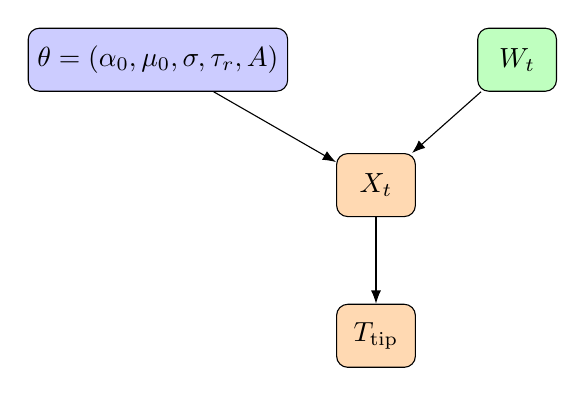
\begin{tikzpicture}[
>=Latex, node distance=1cm,
det/.style={draw, rounded corners, fill=blue!20, minimum width=1cm, minimum height=0.8cm},
rand/.style={draw, rounded corners, fill=green!25, minimum width=1cm, minimum height=0.8cm},
mixed/.style={draw, rounded corners, fill=orange!30, minimum width=1cm, minimum height=0.8cm}
]
\node[det] (theta) {$\theta=(\alpha_0, \mu_0, \sigma, \tau_r, A)$};
\node[rand, right=2.4cm of theta] (Wt) {$W_t$};
\node[mixed, below left=1.1cm of Wt] (Xt) {$X_t$};
\node[mixed, below=1.1cm of Xt] (Ttip) {$\Ttip$};
\draw[->] (theta) -- (Xt);
\draw[->] (Wt) -- (Xt);
\draw[->] (Xt) -- (Ttip);
\end{tikzpicture}
\caption{Directed acyclic graph of model \eqref{eq:model}. Blue: purely epistemic
(deterministic but unknown). Green: purely aleatoric. Orange: general uncertain variables,
random given $\theta$ and epistemically uncertain because $\theta$ is.}
\label{fig:dag}
\end{figure}

\noindent The parameter vector $\theta$ is purely epistemically uncertain because the ocean has one true value of $\theta$. The Brownian motion is pure randomness:
it is the aleatoric forcing (due to weather or unknown forces). The state $X_t$ and, consequently, the tipping time
$\Ttip$ combine both types of uncertainties: for a fixed $\theta$ they are genuine random variables with a probability law, but that law is indexed by an unknown deterministic parameter. \\

\begin{tcolorbox}
\center \textbf{Hypothesis:} Including noise-induced tippings should produce, for the
distribution of $\Ttip$, a left-skewed bell curve: the right tail is cut off by the bifurcation, since tipping is certain
once $t\ge t_c(\theta)$, while the left tail is fed by early escapes whose contribution is
weighted by the epistemic uncertainty about $t_c$.
\end{tcolorbox}

%-------------------------------------------------------------------------------
\subsection{Constructing the posterior}
\label{sec:posterior}
%-------------------------------------------------------------------------------


% inclure ça dans uncertainty modelling et mettre les détails des formules de likelihood dans la partie AMOC article. 

We want to construct a likelihood that avoids resorting to plug-in estimation. \\

\noindent Let $X_S=(x_0,\dots,x_{1924})$ denote the observations before $t_0=1924$ and
$X_N=(y_{1924},\dots,y_{2020})$ those after, both sampled at $\Delta t$ (monthly, $\Delta t=1/12$ year). We keep the same likelihood approximations as defined by the authors. This means that $X_S$ is described by $L_{OU}$ (the Orstein-Uhlenbeck likelihood) and $X_N$ is described by $L_{pseudo}$ (the pseudo-likelihood from Stran splitting). Moreover, let $\Theta = [1, 5] \times [0, 1] \times [0.01, 1] \times [100, 220] \times [0.1, 2.0] $ be the parameter space. \\

\noindent We know that $A$ and $\tau_r$ are non-identifiable on $X_S$, but $\alpha_0$, $\mu_0$ and $\sigma$ are identifiable on both $X_S$ and $X_N$. We can define the following joint likelihood:
\begin{equation}
\label{eq:joint}
L_{\mathrm{all}}(\theta\mid X)=
L_{\mathrm{OU}}\big(\alpha_0,\mu_0,\sigma\mid X_S\big)\cdot
L_{\mathrm{pseudo}}\big(\theta\mid X_N\big),
\end{equation}
which is legitimate because the two blocks of data are separated in time and the process is
Markov, so the full likelihood factorises exactly as the product of the two conditional
likelihoods. Moreover, we choose the uninformative prior equal to 1 on the parameter space $\Theta$. The possibilistic posterior is then:
\begin{equation}
\label{eq:posterior}
f_{\mathrm{all}}(\theta\mid X)=
\frac{L_{\mathrm{all}}(\theta\mid X)}
{\sup_{\theta'\in\Theta}L_{\mathrm{all}}(\theta'\mid X)} .
\end{equation}


\noindent The uninformative possibilistic prior is a crucial element. 
The stationary data carry \emph{no information whatsoever} about $A$ and $\tau_r$. The correct statement of our state of knowledge after seeing
$X_S$ alone is therefore: "the data provide no evidence against any value of $A$ and
$\tau_r$". In the possibilistic framework this is written exactly, as $f_{A,\tau_r}\equiv1$ on
the admissible domain, and it remains a proper description. In the Bayesian framework it
cannot be written: an improper flat prior is not a probability measure and could make the Bayesian evidence (the integral in the denominator) diverge. 

\begin{tcolorbox}
\center The knowledge / ignorance about $A$ and $\tau_r$ must not be modified by the stationary data. A uninformative possibilistic prior achieves this exactly.
\end{tcolorbox}

\noindent To solve the optimization problem in the denominator, we used the algorithm "L-BFGS-B" from Scipy. \\

\noindent In probability theory, the marginal are obtained by integrating with respect to other parameters. In the extension of possibility theory used by J. Houssineau, likewise, we take the supremum with respect to other variables:
\[
f_{\theta_j}(\theta_j\mid X)=\sup_{\theta_{-j}}f_{\mathrm{all}}(\theta\mid X),
\]
Figure \ref{fig:joint_marg} shows the resulting marginal possibility functions. When the peak of the possibility function is quite curved like for $\tau_r$, the epistemic uncertainty is greater. For $\mu_0$ and $\sigma$. 

\begin{figure}[htbp]
\centering
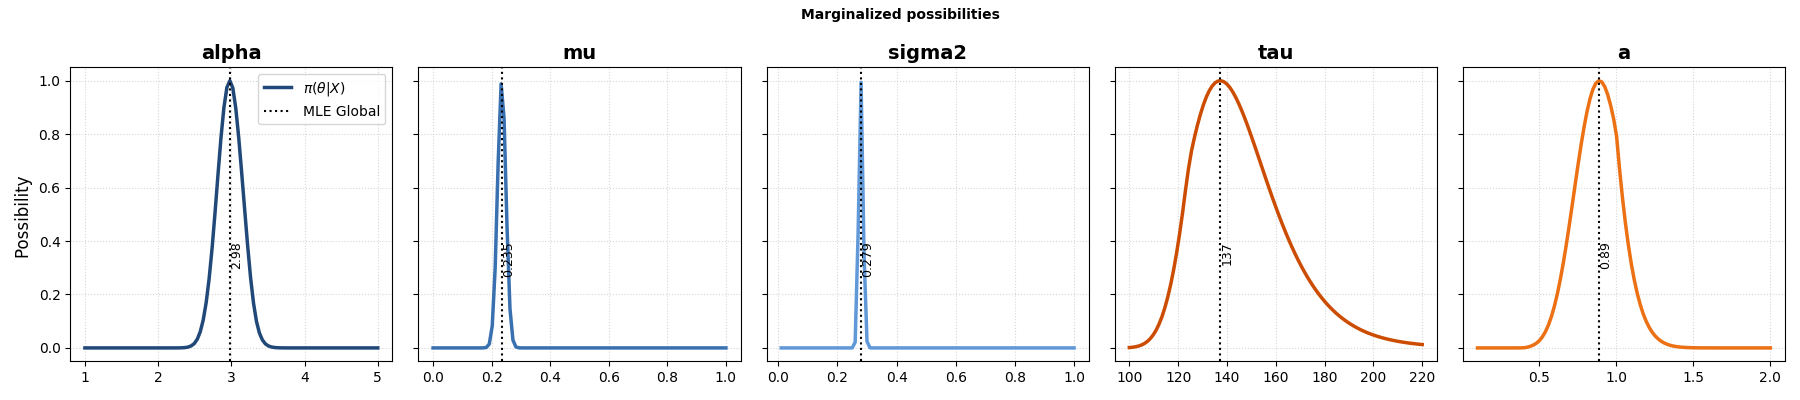
\includegraphics[width=\textwidth]{images/joint_marg.png}
\caption{Marginal possibility functions of the parameters.}
\label{fig:joint_marg}
\end{figure}

\noindent Table \ref{tab:params} compares the possibilistic estimates (the maximum argument of the posterior) with
the maximum likelihood estimates of \cite{ditlevsen2023}. The results are quite similar. This seems to indicate that the plug-in estimation they used did not have a serious influence on the other estimates. This is not surprising given the marginals of $\alpha_0$, $\mu_0$ and $\sigma$ because they are very concentrated on the mode, which means the data provided very little uncertainty / strong confidence on these parameters. \\

\begin{table}[htbp]
\centering


\small
\begin{tabular}{lcccccccc}
\toprule
 & $\alpha_0$ & $\mu_0$ & $\sigma$ & $\tau_r$ & $A$ & $m$ & $\lambda_0$ & $t_c$ \\
\midrule
Article \cite{ditlevsen2023} & 3.06 & 0.25 & 0.55 & 140.63 & 0.86 & $-1.54$ & $-2.73$ & 2064.63 \\
Possibility (this work) & 2.98 & 0.23 & 0.53 & 137.18 & 0.89 & $-1.44$ & $-2.49$ & 2061.18 \\
\bottomrule
\end{tabular}
\caption{Parameter estimates: two-step maximum likelihood of \cite{ditlevsen2023} versus modes
of the joint possibilistic posterior \eqref{eq:posterior}.}
\label{tab:params}
\end{table}


%-------------------------------------------------------------------------------
\subsection{Including noise-induced tipping}
\label{sec:noise}
%-------------------------------------------------------------------------------

\subsubsection{The right quantity to estimate}

The \emph{effective tipping time} is not given by $t_c$, but by:
\begin{equation}
\label{eq:ttip}
\Ttip:=\inf\Big\{t\ge t_0:\ X_t\le x_u(\lambda_t)=m-\sqrt{-\lambda_t/A}\Big\},
\end{equation}
the first time the trajectory crosses the moving unstable branch and enters the collapsed
basin. By construction $\Ttip\le t_c$ almost surely, because the unstable branch merges
with the stable one at $t_c$. \\

\noindent Two mechanisms can trigger \eqref{eq:ttip}. A \emph{bifurcation-induced} (b-tipping) event
occurs when the barrier disappears (at $t_c)$; a \emph{noise-induced} (n-tipping) event occurs when a
fluctuation carries the state over the potential barrier that before $t_c$. Figure \ref{fig:MC_tip} shows what happens when \eqref{eq:ttip} is recorded in the Monte Carlo simulations. \\

\noindent A third mechanism,
\emph{rate-induced} tipping \cite{ashwin2012} (r-tipping), in which the equilibrium moves faster than the
state can track it, can be excluded here on two grounds. Quantitatively, the ramping speed is
$|\dot\lambda|=|\lambda_0|/\tau_r\approx 2.49/137\approx1.8\times10^{-2}$ per year, which is slow compared to the system's mechanisms. Qualitatively,
r-tipping is defined by a failure to track an equilibrium that continues to exist, whereas here
the equilibrium disappears after bifurcation. \\

\begin{figure}[htbp]
\centering
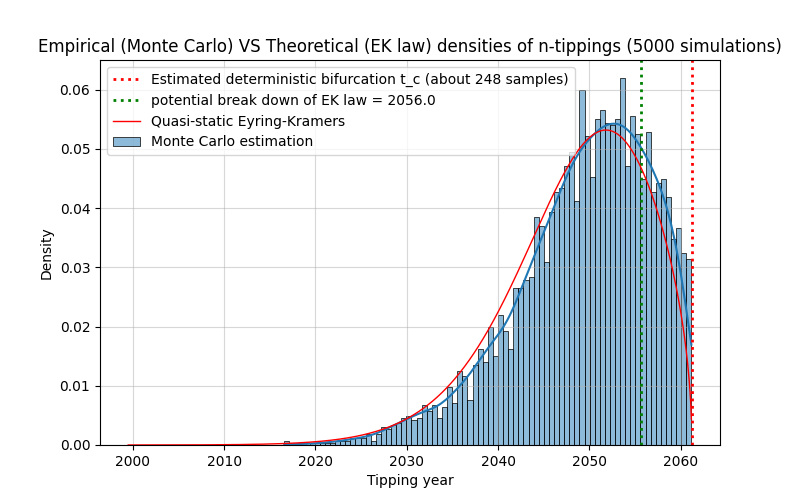
\includegraphics[width=\linewidth]{images/MC_tip.png}
\caption{Distribution of the effective tipping time $\Ttip$ over $5000$ simulations of model
\eqref{eq:model} with the estimated parameters from the possibilistic posterior, separating noise-induced from
bifurcation-induced events. With $t_c=2061.2$, one obtains $\Ttip\in[2032,\,2061.25]$ at
$95\%$, and the large majority of the trajectories tip before the bifurcation.}
\label{fig:MC_tip}
\end{figure}

\noindent More than 80\% of the simulated trajectories tip before $t_c$. The interval $[2037,2109]$ published in
\cite{ditlevsen2023} is an interval for a quantity that, with high probability, will never be
observed, because the collapse will have occurred earlier. Under the same model, we obtain $\Ttip\in[2032,\,2061.25]$ at
$95\%$ confidence level. 

\subsubsection{A non-homogeneous escape rate}

To make this analytical rather than purely numerical, we model the noise-induced escape as the
first event of a non-homogeneous Poisson process. We extend the Eyring-Kramers law to a quasi-static setup. Considering $\lambda_t$ constant between each observation, we can compute \eqref{eq:ek} for the mean waiting time
in the resulting fixed potential at each time $t$. This defines a time-dependent escape rate:
\[
r(t\mid\theta):=\frac{1}{\tau_n(\lambda_t\mid\theta)}.
\]

\noindent We can finally write that the probability of tipping given $\theta$ is:
\begin{equation}
\label{eq:cdftip}
P\big(\Ttip\le t\mid\theta\big)=
\begin{cases}
1-\exp\Big(-\displaystyle\int_{t_0}^{t}r(s\mid\theta)\,\dd s\Big) & \text{if } t<t_c(\theta),\\[10pt]
1 & \text{if } t\ge t_c(\theta).
\end{cases}
\end{equation}
The hard switch at $t_c(\theta)$ encodes the fact that tipping is certain once the stable state
has disappeared. Figure \ref{fig:mean_tau} shows the evolution of $\tau_n(\lambda_t)$ and
Figure \ref{fig:cdf_EK} the resulting distribution function for a fixed $\theta$.


\begin{figure}[htbp]
\centering
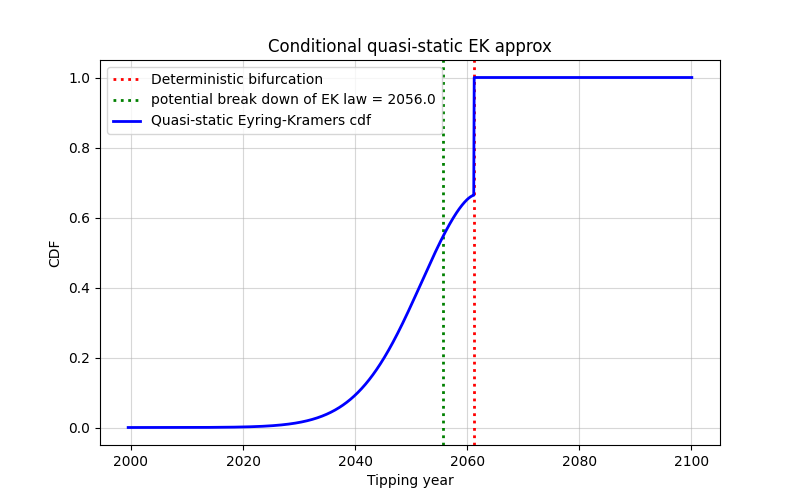
\includegraphics[width=\linewidth]{images/cdf_EK.png}
\caption{Probability $\Prob(\Ttip\le t\mid\theta)$ of observing a tipping before $t$, computed
from \eqref{eq:cdftip} at the possibilistic mode $\theta=\Estar[\theta\mid X]$.}
\label{fig:cdf_EK}
\end{figure}





\subsubsection{Two failures of the quasi-static approximation}

The construction above is convenient but it rests on an asymptotic result, and we identified
two distinct problems with it.

\medskip
\noindent\textbf{Problem 1: the analytical rate disagrees with the empirical one.} Comparing
\eqref{eq:cdftip} with the empirical distribution obtained from $5000$ simulations (Figure
\ref{fig:MC_tip}), even though the shapes are very similar, we notice a discrepancy. The quasi-static Eyring-Kramers approximation is more pessimistic than the empirical density as it gives more weight the previous tipping times (left-skewed). Close to $t_c$, the analytical model assigns roughly $60\%$
probability to a tipping before $t_c$, whereas the simulations give more than $80\%$. The Kolmogorov
distance $D(t)=\sup_{u\le t}|\hat F(u)-F(u)|$ of Figure \ref{fig:kolmo} quantifies the discrepancy
between the two.  \\




\begin{figure}
    \centering
    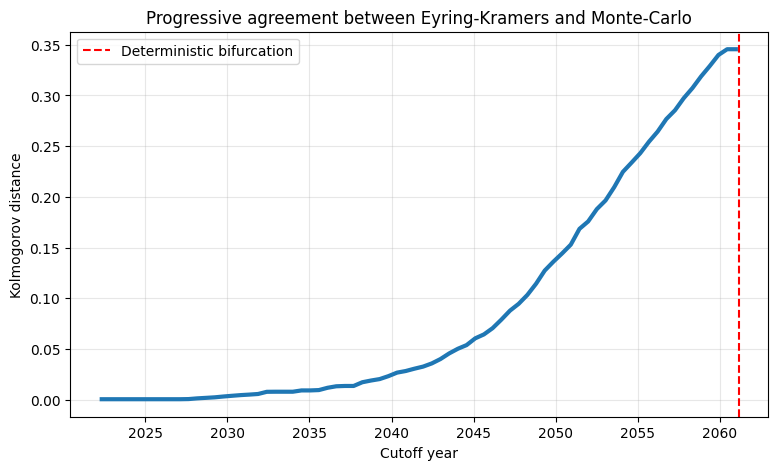
\includegraphics[width=\linewidth]{images/kolmogorov_dist.png}
    \caption{Kolmogorov distance $D(t)=\sup_{u\le t}|\hat F(u)-F(u)|$.}
    \label{fig:kolmo}
\end{figure}

\medskip
\noindent\textbf{Problem 2: the approximation breaks down exactly where it matters.} The mean waiting time before a noise-induced tippings falls by many orders of magnitude as the
barrier $\Delta(\lambda_t)=4|\lambda_t|^{3/2}/(3\sqrt A)$ shrinks. Around $2050$ it is of the
order of ten years. But close from the bifurcation time, this time increases (see \ref{fig:mean_tau}). Which should be the case as the potential barrier is low. This is a failure of the formula as its prediction contradicts simulations. As
$\lambda_t\to0$ the barrier $\Delta(\lambda_t)\to0$ and the prefactor
$\sqrt{V''(\mu)|V''(x_u)|} \to 0$, so that $\tau_n(\lambda_t)\to0$ like
$|\lambda_t|^{-1/2}$. The Eyring--Kramers asymptotics requires
$\Delta(\lambda)\gg\sigma^2$; near $t_c$ this fails, the two fixed points are no longer
separated on the scale of the fluctuations. This is the main mathematical obstacle encountered during the internship. \\

 




\begin{figure}
    \centering
    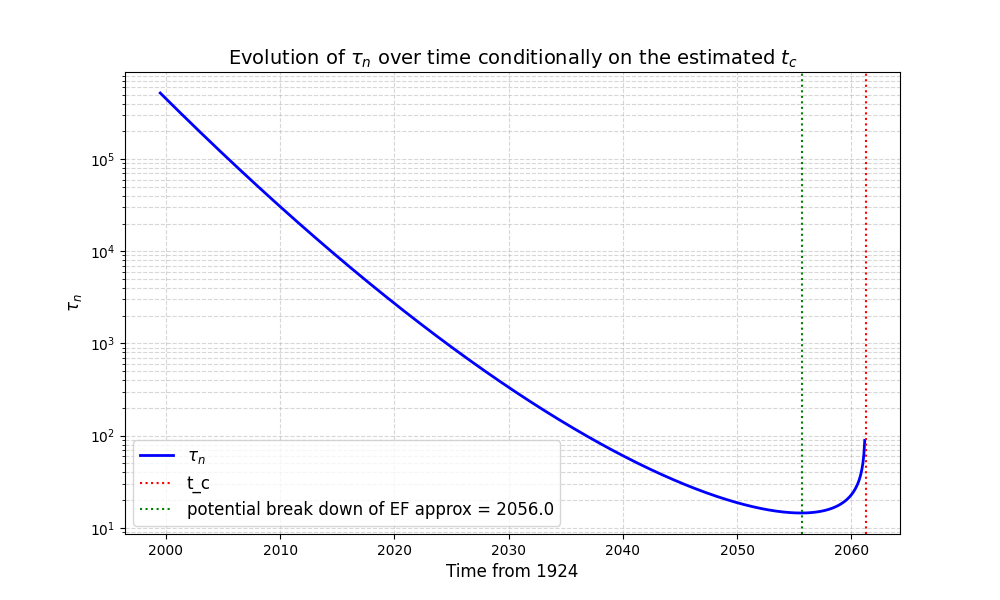
\includegraphics[width=\linewidth]{images/mean_tau_noise_evolution.png}
    
    \caption{Evolution of the mean Eyring--Kramers waiting time $\tau_n(\lambda_t)$ before a
noise-induced tipping, for the estimated parameters.}
    \label{fig:mean_tau}
\end{figure}

\subsection{First results: cumulative possibility and necessity}

Even though the quasi-static Eyring-Kramers law does not give a completely valid result, we can still use it. The credibility that the AMOC has tipped before $t$ is: 
\begin{equation}
\label{eq:opmtip}
\boxed{\;
\Pbar\big(\Ttip\le t\big)=\sup_{\theta\in\Theta}
f_{\mathrm{all}}(\theta\mid X)\cdot P \big(\Ttip\le t\mid\theta\big) \; }
\end{equation}

\noindent The OPM \eqref{eq:opmtip} is an upper bound. Its dual, the necessity, provides a lower bound, defined as: 
\begin{equation}
\label{eq:nec}
N\big(\Ttip\le t\big)=1-\Pbar\big(\Ttip>t\big)
=1-\sup_{\theta\in\Theta}f_{\mathrm{all}}(\theta\mid X)\,
\Big(1-\Prob\big(\Ttip\le t\mid\theta\big)\Big),
\end{equation}
is the corresponding lower bound, and the pair
$\big[N(\Ttip\le t),\ \Pbar(\Ttip\le t)\big]$ is a \emph{probability interval} for the
distribution function of the tipping time: any probabilistic model compatible with the
available information assigns to $\{\Ttip\le t\}$ a probability inside this interval. The width
of this interval is a reflection of the epistemic uncertainty: the wider it is, the greater the epistemic uncertainty. \\


\noindent Figure \ref{fig:possTip} displays the credibility and necessity. Again, the credibility is not a probability distribution function
and must not be read as one: $\Pbar(\Ttip\le t)$ is the credibility of the event, that is the
largest probability attainable by a parameter that the data do not contradict, each candidate
being discounted by its posterior possibility. \\

\begin{figure}[htbp]
\centering
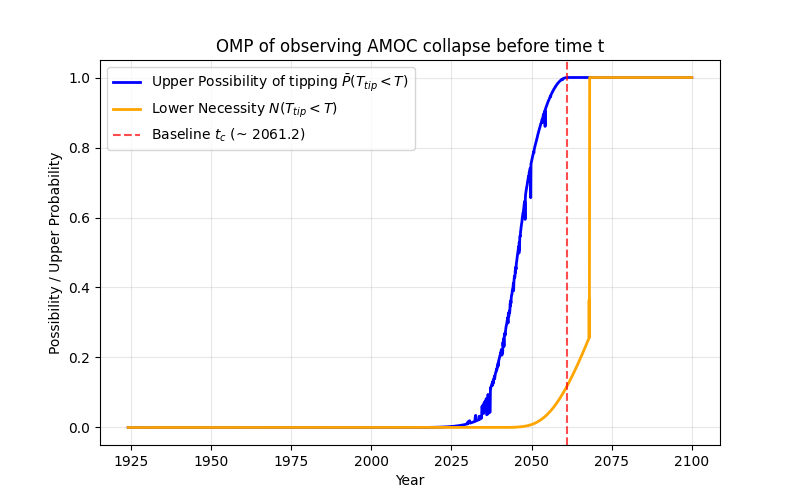
\includegraphics[width=\linewidth]{images/possTip.png}
\caption{Cumulative credibility and necessity of tipping. The little artifacts on the credibility curve are due to hard optimization problem and arise from a time discretization that was too precise}
\label{fig:possTip}
\end{figure}

\noindent Two structural difficulties of \eqref{eq:opmtip} appear. First, the threshold
$t_c(\theta)$ moves \emph{inside} the optimization: the objective is discontinuous in $\theta$
when $\{t_c(\theta)=t\}$, which makes gradient-based optimization delicate. Second, the hard threshold in \eqref{eq:cdftip}
sits uneasily with the soft epistemic weighting: for $t$ slightly beyond the most credible
$t_c$, the supremum is attained by parameters whose $t_c$ is just below $t$, so the curve is
driven by the tail of the posterior rather than by its mode. This is a not a bug. \\

\noindent Out of curiosity, we plotted the evolution of the maximizer during the credibility computations (see \ref{fig:evolparams}). This was never studied before so there is still no fixed interpretation. in a more general situation, the dynamic evolution of the parameters with the possibility value (calculated from the marginals) might help us better understand why some results might be weird or harder to interpret due to an increase in uncertainty for one parameter. Except the optimization artifacts, we notice that the parameters $\tau$ and $A$ exhibit a strong epistemic uncertainty between 2000 and 2025. 


\begin{figure}[htbp]
\centering
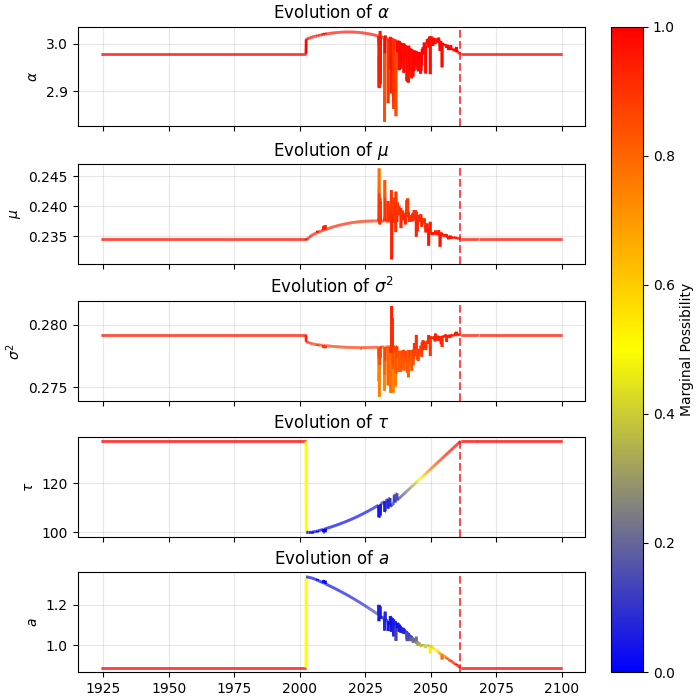
\includegraphics[width=\linewidth]{images/evol_params.png}
\caption{Trajectory of the maximizing parameter $\theta^\star(t)$ during the computation of credibility (\eqref{eq:opmtip}), with a color indicating the value of the marginal possibility associated to each parameter (1 means possible, 0 means impossible).}
\label{fig:evolparams}
\end{figure}


\noindent A last, more speculative point. In the simulations we classify each tipping as noise-induced or
bifurcation-induced by comparing $\Ttip$ with $t_c(\theta)$. But $t_c$ is epistemically
uncertain: a tipping labeled ``noise-induced'' under one credible parameter value would be
labeled ``bifurcation-induced'' under another. The label is therefore not a property of the
trajectory but of the pair (trajectory, parameter). Two ways out are conceivable. how to differentiate between them? This is still an open question. \\

%-------------------------------------------------------------------------------
\subsection{Taking a step back: is tipping the right object?}
\label{sec:stepback}
%-------------------------------------------------------------------------------

The definition \eqref{eq:ttip} treats the first crossing of the unstable branch as an
irreversible event. In the deterministic dynamics it is: once past $x_u$, the drift pushes the
state towards $-\infty$. In the stochastic dynamics it is not. A trajectory that crosses the
barrier early, when the barrier is still shallow relative to the noise, can be pushed back by
a subsequent fluctuation and return to the neighborhood of the stable branch. We modify the code to capture such scenarios. Figure
\ref{fig:circ} shows the classification of the $1000$ simulated trajectories into the four
resulting categories, and Figures \ref{fig:ex1}--\ref{fig:ex4} give one representative example
of each.

\begin{figure}[htbp]
\centering
\begin{minipage}{0.42\textwidth}
Because of the randomness, and for a fixed $\theta$, some trajectories that have crossed the
barrier return to the stable region. About $84\%$ of the simulations tipped before $t_c$ in the
sense of a crossing that was \emph{not} followed by a return. The discrepancy with the $60\%$ predicted by the escape-rate model
\eqref{eq:cdftip} might just be a genuine failure of the
quasi-static approximation.


\end{minipage}\hfill
\begin{minipage}{0.55\textwidth}
\centering
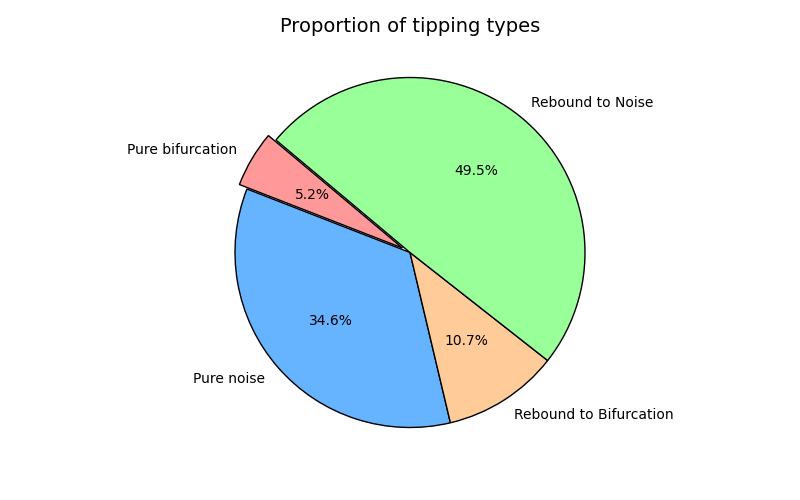
\includegraphics[width=\linewidth]{images/circular_tip_phenom.png}
\end{minipage}
\caption{Classification of the simulated trajectories according to the mechanism of the
crossing and to whether a return to the stable region occurred.}
\label{fig:circ}
\end{figure}

\begin{figure}[htbp]
\centering
\begin{subfigure}[b]{0.47\textwidth}
\centering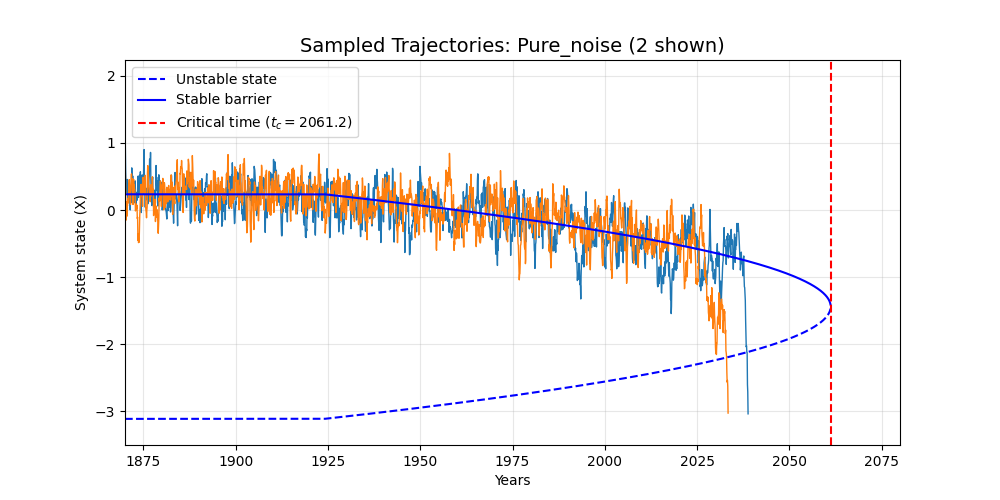
\includegraphics[width=\textwidth]{images/example_Pure_noise.png}
\caption{Pure noise-induced tipping.}\label{fig:ex1}
\end{subfigure}
\hfill
\begin{subfigure}[b]{0.47\textwidth}
\centering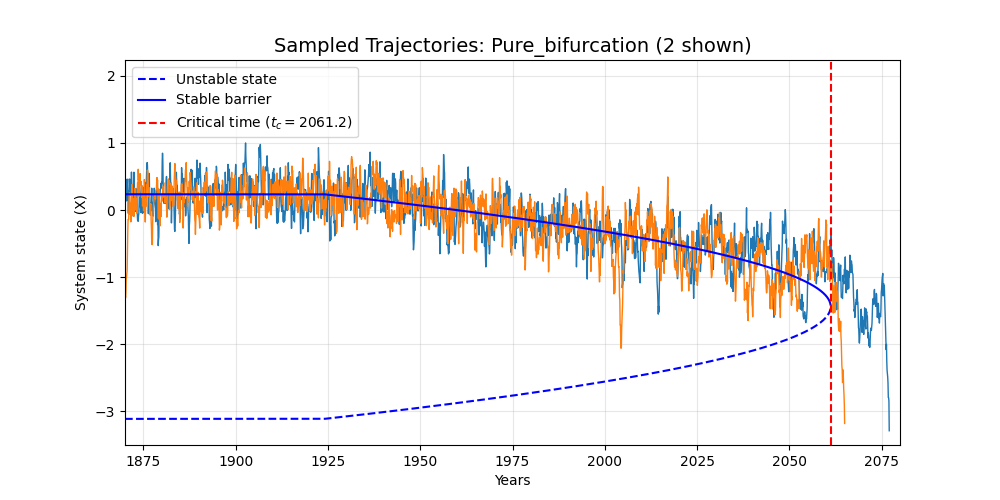
\includegraphics[width=\textwidth]{images/example_Pure_bifurcation.png}
\caption{Pure bifurcation-induced tipping.}\label{fig:ex2}
\end{subfigure}

\vspace{0.35cm}
\begin{subfigure}[b]{0.47\textwidth}
\centering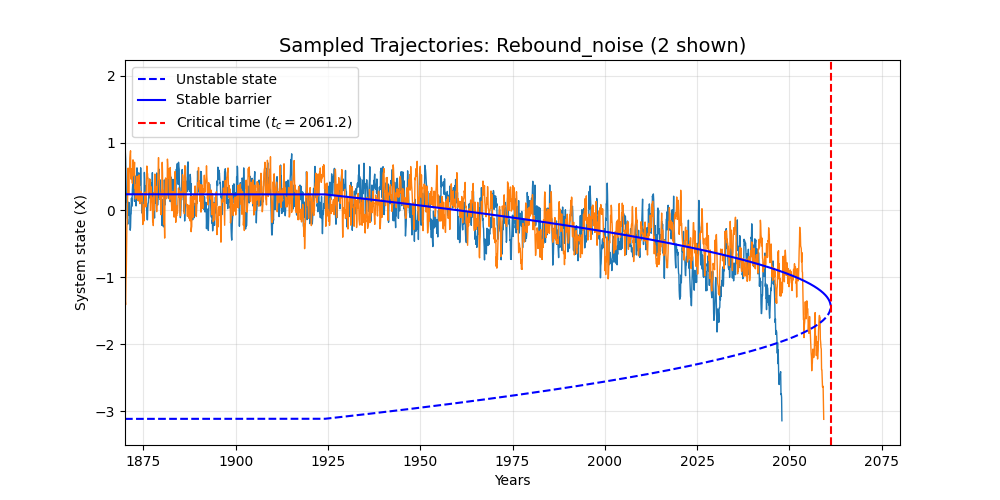
\includegraphics[width=\textwidth]{images/example_Rebound_noise.png}
\caption{Crossing followed by a return, then noise-induced tipping.}\label{fig:ex3}
\end{subfigure}
\hfill
\begin{subfigure}[b]{0.47\textwidth}
\centering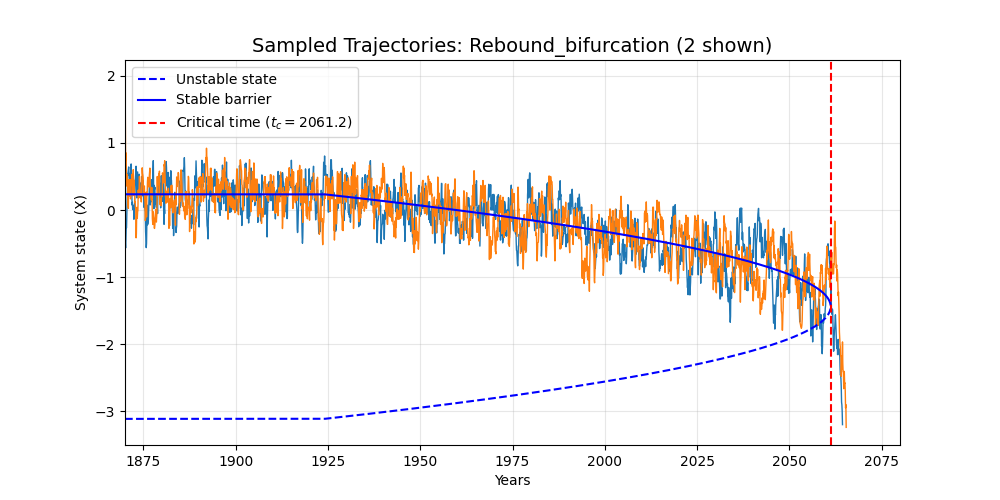
\includegraphics[width=\textwidth]{images/example_Rebound_bifurcation.png}
\caption{Crossing followed by a return, then bifurcation-induced tipping.}\label{fig:ex4}
\end{subfigure}
\caption{Four representative trajectories illustrating the possible tipping behaviours.}
\label{fig:examples}
\end{figure}

\noindent This raises a legitimate objection to the whole study. If the state can return, the first
passage time is not the physically meaningful quantity; one should rather study the occupation
time of the collapsed basin, or the probability of being in the collapsed state at a given
date. In the real ocean the question is even less clear-cut, since a partial and temporary
weakening is not the same event as a complete shutdown \cite{rahmstorf2005}. \\

\noindent We have deliberately chosen not to pursue this direction. Deciding what quantity to study is a question for climatologists rather than statisticians. Our contribution concerns the treatment of uncertainty in a \emph{given}
model, and changing the model at the same time would make it impossible to attribute the
differences with \cite{ditlevsen2023} to the inferential machinery. We therefore keep the
first-passage definition and record the returns as a caveat rather than as a correction. \\



\bigskip


%%%%%%%%%%%%%%%%%%%%%%%%%%%%%%%%%%%%%%%%%%%%%%%%%%%%%%%%%%%%%%%%%%%%%%%%%%%%%%%
\section{Perspectives}
\label{sec:perspectives}
%%%%%%%%%%%%%%%%%%%%%%%%%%%%%%%%%%%%%%%%%%%%%%%%%%%%%%%%%%%%%%%%%%%%%%%%%%%%%%%

\subsection{Continuation of the AMOC collapse estimation}
\label{sec:amoc-continuation}

The work reported in Section \ref{sec:contrib} is at the stage where the methodology is in
place, the main qualitative conclusion is established (noise-induced tipping dominates and
shifts the credible tipping a decade earlier) and the remaining tasks are those that
separate a set of results from a publishable article. In order of priority:

\begin{enumerate}
\item \textbf{Replace the Eyring--Kramers approximation near the bifurcation.} This is the main
technical gap, and is developed in Section \ref{sec:fp} below.

\item \textbf{Tackle the uncertainty on the likelihood approximations.} The joint likelihood comes from a linearization and a computational scheme (Strang splitting). We did not estimate the parameters with the likelihood from the true model. Maybe this can affect results. 

\item \textbf{Writing the article.} The natural target is a journal at the interface between statistics and
climate science. The goal is to show a proof of concept of possibility theory and the importance of accounting for ignorance.
The argument has to be made in a way that a climatologist and statistician can act on. \\
\end{enumerate}


\subsubsection{Fokker--Planck equation}
\label{sec:fp}

\noindent The cleanest way to remove the Eyring--Kramers error near $t_c$ is to abandon the asymptotic
formula and to solve the first-passage problem directly. We can obtain the density of the stopping time $\Ttip$ thanks to the Fokker-Planck equation. We just need to set an absorbing condition
on the unstable branch:
\begin{equation}
\label{eq:fp}
\begin{cases}
\partial_t p(x,t)=2A(x-m)\,p(x,t)+\big(A(x-m)^2+\lambda_t\big)\partial_x p(x,t)
+\dfrac{\sigma^2}{2}\partial_{xx}p(x,t),\\[8pt]
p(x,t)=0 \quad\text{for}\quad x=m-\sqrt{-\lambda_t/A},
\end{cases}
\end{equation}
and the density of the tipping time is obtained from the survival function
\begin{equation}
\label{eq:survival}
S(t)=\int_{m-\sqrt{-\lambda_t/A}}^{+\infty}p(x,t)\,\dd x,
\qquad f_{\Ttip}(t)=-\frac{\dd S}{\dd t}(t).
\end{equation}

\noindent Notice that, can rewrite the the first equality as $\partial_t p(x, t) = - \partial_x J(x,t)$ with $J(x, t)= b(x,t) \cdot p(x,t) - \frac{\sigma^2}{2} \partial_x p(x,t)$ and $b(x,t) = -(A(x-m)^2 + \lambda_t)$. This notation will be usefull for later computations.  \\

\noindent This formulation is exact: it makes no small-noise assumption and it handles the moving
boundary natively, at the price of a numerical solution. We can replace the imprecise condition "$\Delta(\lambda) \gg \sigma$" by precise numerical bounds. This enables us to Replace an uncontrolled asymptotic error by a controllable discretization
error. \\

\noindent This Fokker-Planck equation is however very difficult to solve. It is a second order differential equation that is not homogeneous in time with a moving border condition. Having no experience with numerical algorithms to solve differential equation, this part will be quite hard. A solution might be to use recent agentic systems for scientific computing, such as
the ATHENA framework developed by G. E. Karniadakis, which automates the derivation
and the implementation of PDE solvers; the interest for us is less the automation than the
possibility of generating and cross-validating several independent discretizations of
\eqref{eq:fp}, which gives an empirical handle on the numerical error. \\

\paragraph{Landau transform:} We can simplify the equation by removing the moving boundary given in the Dirichlet condition. This is called a Landau transform of the function $p$. If we write $l(t) : = m - \sqrt{-\lambda_t / A}$ and $r=3$ as an upper bound on the values of $X_t$, we can let $y(t) := \frac{x - l(t)}{L(t)}$, where $L(t) = r - l(t)$. We also add another boundary condition $J(r,t) = 0$ (the flux of probability at the boundary given by the upper bound on $X_t$ should be zero). \\

\noindent By setting the following change of variable $q(y,t)dy = p(x,t)dx$, we get that the survival probability is now given by an integral whose boundaries are constant with respect to time: $S(t) = \int_{l(t)}^r p(x,t) \dd x = \int_0^1 q(y, t) \dd y$. \\

\noindent Moreover, we get: $\partial_t q(y, t) = - \partial_y \tilde{J}(y,t)$, where $\tilde{J}(y,t) := \frac{\tilde{b}(y,t)}{L(t)} q(y,t) - \frac{\sigma^2}{2} \cdot \frac{1}{L(t)^2} \partial_y q(y,t)$, with $\tilde{b} = b(x(y,t), t) - l'(t)(1-y)$.  We also have two boundary equalities: $q(0,t) = 0$ and $\tilde{J}(r,t) = 0$. \\

\begin{proof}
First note that $q(y,t) = p(x,t) L(t) \implies \partial_x p(x,t) = \frac{1}{L} \partial_x q(y,t) = \frac{1}{L^2} \partial_y q(y, t)$. \\

\begin{align}
    \partial_t q(y, t) &= \partial_t ((x,t)  L(t)) \\
    &= \partial_t p(x,t)  L(t) + p(x,t)  \partial_t L(t) \\
    &= - \partial_x (J(x,t)  L(t)) - p(x,t)  l'(t) \\
    &= - \partial_x (J(x,t)  L(t)) - \frac{1}{L}l'(t)q(y,t)
\end{align}

Rewriting $J$ with $q$ we get: 
\begin{align}
J(y,t) &= \frac{b(y,t)}{L(t)}q(y,t) - \frac{\sigma^2}{2} \cdot \frac{1}{L(t)^2} \partial_y q(y,t) \\
&= \tilde{J}(y,t) + \frac{1}{L}l'(t)(1-y)q(y,t) 
\end{align}

This implies:
\begin{align}
    - \partial_x(J(x,t) L(t)) &= -\partial_x( \tilde{J}(y,t)L(t) + \frac{1}{L}l'(t)(1-y)q(y,t)  \\
    &= \partial_y \tilde{J}(y,t) - l'(t) \partial_x(q(y,t) - y q(y,t)) \\
    &= \partial_y \tilde{J}(y,t) + \frac{1}{L}l'(t)q(y,t)
\end{align}

Therefore
$$
\partial_t q(y,t) = - \partial_y \tilde{J}(y,t) + \frac{1}{L}l'(t)q(y,t) - \frac{1}{L}l'(t)q(y,t) = - \partial_y \tilde{J}(y,t)
$$

Regarding the boundary conditions, we have $q(0,t) = 0$ because $y=0 \implies x(0,t) = l(t)$ and $p(l(t), t) = 0, \forall t$. When $y=1$, $x(1,t) = r, \forall t$. 
$$
\tilde{J}(1,t) = J(r,t) - + \frac{1}{L}l'(t)(1-1)q(y,t) = 0
$$

    
\end{proof}

\noindent Finally, we get that the density of $\Ttip$ is given by:
$$
- S'(t) = - \int_0^1 \partial_t q(y,t) \dd y = - \tilde{J}(1,t) + \tilde{J}(0,t) = \tilde{J}(0,t).
$$




\subsubsection{Uncertainty on likelihoods}
\label{sec:omega}

\begin{quote}
\small
``Use of the pseudo-likelihood in place of the true likelihood function in a maximum likelihood
analysis can lead to good estimates, but \textbf{a straightforward application of the usual
likelihood techniques to derive information about estimation uncertainty, or for significance
testing, would in general be incorrect}.'' \hfill--- Dodge \cite{dodge2003}
\end{quote}

\noindent Everything above rests on two approximations: the linearization of the drift in the stationary
phase, and the Strang splitting in the non-stationary phase. Neither is the true likelihood.
We would like to quantify how these likelihood deviates from the true likelihood. \\

\noindent The problem is that these quantifications can become quite difficult mathematically. For the deviation between the true likelihood on stationary data and the Orstein-Uhlenbeck likelihood, we could start from the KL-divergence and use some theorems like Girsanov's theorem to simplify the computations. \\

\noindent Strang splitting (\cite{pilipovic2024}) is a recent computational scheme and the theoretical bounds we can find are not directly applicable to the quantification of likelihood deviation. \\

\noindent Even if we succeed to obtain bounds on likelihood deviations, how can we use them in the probabilistic-possibilistic framework? Maybe these bound could be put inside the optimization problem, under a form that penalized values of parameters that increase likelihood deviation. \\

\noindent A technique from possibility theory might bring a solution. We can flatten the posterior by using an exponent $\omega$ whose value is lesser than 1. The supremum of the posterior will still be 1, so we still get a valid possibility function. Flattening the possibility function means making the epistemic uncertainty greater everywhere. As our likelihood is uncertain, we might as well make the posterior more uncertain too. This could avoid very complex calculations to obtain theoretical bounds on likelihood deviations. But this raises a new question: how to choose $\omega$? A first idea might be to generate many simulations for different values of $\omega$, and select the value for which the generated simulations are the closest from real data. But our data is limited as it stops at $t=2020$. \\

\newpage



\paragraph{Mis-specified M-estimation with possibility theory:} 

%juste show how KL appears, what we want, Bregman divergence, fisher information ...

We want to quantify the deviation between the true distribution and the approximated distributions (linearization on the stationary regime, Strang splitting on the non-stationary regime). Let $P_\theta := \mathcal{L}((X_t)_{t \in [1870, 2020]}$ be the true path distribution of the stochastic process on $[1870, 2020]$ given a value of the deterministic uncertain variable $\bm{\theta}$. Let $Q_\theta$ be the path distribution of the linearized process and $S_\theta$ be the path distribution obtained from Strang splitting. \\

% QUESTION: HOW CAN I COMBINE BOTH UNCERTAINTIES ??????????? THE LIKELIHOOD IS DEFINED ON ALL THE DATA

\noindent In the mis-specified settings, if $f$ is the true model and $g$ is the model used to approximate it, we obtain the 2 following properties regarding Maximum Likelihood Estimation:
\begin{enumerate}
    \item $\frac{1}{n}\sum_{i=1}^{n} \log g(X_i) \to  \mathbbm{E}_f[\log g(X)]$.
    \item $\mathbbm{E}_f[\log f] = \mathbbm{E}_f[\log g] + D_{KL}(f || g)$. \\
\end{enumerate}

\noindent Finally, we get that if $\theta^*$ is the true parameter, $\psi$ is the theoretical parameter value from the approximated likelihood and $\hat{\psi}_n$ is the MLE estimate, we can decompose the error into an approximation error and a finite sample error (the latter is guaranteed to be $O(n^{-1/2}))$:
$$
|| \theta^* - \hat{\psi}_n|| = || (\theta^* - \psi) + (\psi - \hat{\psi}_n)||.
$$

\noindent The approximation error is hard to quantify. The goal is to bound the KL divergence and use the Bregman divergence with an approximation relying on the Fisher information to translate the bound into uncertainty intervals for the parameters. \\

\paragraph{Quantifying the deviation from the true and the linearized distributions:}

\noindent Let $W_t^{P_\theta}$ and $W_t^{Q_\theta}$ be the Brownian motion for the distribution $P_\theta$ and $Q_\theta$ respectively. We have:
\begin{align}
    dX_t &= -(A(X_t - m)^2 + \lambda_0)dt + \sigma dW_t^{P_\theta} \\
    & \approx - \alpha(X_t - \mu)dt + \sigma dW_t^{Q_\theta}
\end{align}

\noindent First, let $\mu_0 = \mu(\lambda_0)$, $b(x) = -A(x - m)^2 - \lambda_0$ and $\tilde{b} = -2A(x - m)$ (the linearized drift around the stable fixed point $\mu_0$). The difference between the drift and linearized drift is: $|b(x) - \tilde{b}(x)| = A(x - \mu_0)^2, \forall x$. \\

To bound the KL divergence, we need Girsanov's theorem. We first need to characterize $W_t^{Q_\theta}$. 
\begin{align}
    & b(X_t)dt + \sigma dW_t^{P_\theta} = \tilde{b}(X_t)dt + \sigma dW_t^{Q_\theta} \\
    &\implies dW_t^{Q_\theta} = dW_t^{P_\theta} + \frac{b(X_t) - \tilde{b}(X_t)}{\sigma}dt \\
    & \implies W_t^{Q_\theta} = W_t^{P_\theta} + \int_0^t \frac{b(X_s) - \tilde{b}(X_s)}{\sigma}ds
\end{align}


By Girsanov's theorem, we have:
$$
\frac{\dd Q_\theta}{\dd P_\theta} = \exp \left( \int_0^t \frac{b(X_s) - \tilde{b}(X_s)}{\sigma}dW_s^{P_\theta} - \frac{1}{2} \int_0^t \big( \frac{b(X_s) - \tilde{b}(X_s)}{\sigma} \big)^2ds \right)
$$

Therefore, assuming we have the right conditions (weak assumptions) to ensure that the stochastic integral inside the exponential is a martingale, the Kullback-Leibler divergence reduces to: 
\begin{align}
    D_{KL}(P_\theta || Q_\theta) &= - \mathbbm{E}_{P_\theta} \left[ \log \frac{dQ_\theta}{dP_\theta} \right] \\
    &= -\mathbbm{E}_{P_\theta} \left[ \int_0^t \frac{b(X_s) - \tilde{b}(X_s)}{\sigma}dW_s^{P_\theta} \right] + \frac{1}{2} \mathbbm{E}_{P_\theta} \left[ \int_0^t \big( \frac{b(X_s) - \tilde{b}(X_s)}{\sigma} \big)^2ds \right] \\
    &=  \frac{A^2}{2 \sigma^2} \mathbbm{E}_{P_\theta} \left[ \int_0^t (X_s - \mu_0)^4ds \right] \\
    &= \frac{A^2}{2 \sigma^2} \int_0^t \mathbbm{E}_{P_\theta}[(X_s - \mu_0)^4]ds
\end{align}


% sure about that ??????????????
We need to find a bound on the fourth moment of $X_t$. \textbf{Conditioning on $X_0 = \mu_0$}, notice that: 
$$
X_s - X_0 = \int_0^s b(X_u)du + \int_0^s \sigma dW_u^{P_\theta}
$$

We know that for $a,b \in \mathbbm{R}$, $(a+b)^4 \leq 8(a^4 + b^4)$. Therefore:
$$
\mathbbm{E}_{P_\theta}[(X_s - X_0)^4] \leq 8\mathbbm{E}_{P_\theta} \big[ \big( \int_0^s b(X_u)du \big)^4 \big] + 8\mathbbm{E}_{P_\theta}\big[\big(\int_0^s \sigma dW_u^{P_\theta}\big)^4\big] \\
$$

The second term is just the expectation of the fourt moment of a random variable with distribution $\mathcal{N}(0, s\sigma^2)$. Regarding the first term, we can use Hölder's inequality. Let $f$ be an integrable function. We have $\big( \int_0^s f(u)du \big)^4 \leq  s^3 \int_0^s f(u)^4du$. Assuming that the drift is bounded by $K \in \mathbbm{R}$, we get:
$$
\mathbbm{E}_{P_\theta}[(X_s - X_0)^4] \leq 8K^4s^4 + 24 \sigma^4s^2
$$

So, by integrating, we finally get: 
\begin{equation}
    D_{KL}(P_\theta || Q_\theta) \leq \frac{4}{5} \frac{A^2}{\sigma^2}K^4t^5 + 8\sigma^4t^3.
\end{equation}

Let's call the quantity $\frac{4}{5} \frac{A^2}{\sigma^2}K^4t^5 + 8\sigma^4t^3$ as $B(t)$ (for "bound")

\paragraph{From a bound on $D_{KL}$ to a bound on parameters:} To translate the bound on the Kullback-Leibler divergence, we resort to the Bregman divergence. Let $p_\eta$ be a density from the exponential family, parametrized with $\eta$ and with $A$ a strictly convex function, namely $p_\eta(x) = h(x) \exp( \langle \eta, T(x) \rangle - A(x))$. In this case, we have an equality between the Kullback-Leibler divergence and the Bregman divergence:
$$
D_{KL}(p_{\eta_1} || p_{\eta_2}) = B_A({\eta_2}, {\eta_1}).
$$


We can create a new parametrization so that the true model and the linearized model can both be expressed the same way by different parameters. For example, under a polynomial parametrization $\mathcal{M} = \{P_\beta: \beta \in \mathbbm{R}^3\}$, the true model corresponds to the parameter $\beta = (Am^2 - \lambda_0, -2Am, -A)$ (for which we still have identifiability) and the linearized model to $\gamma = (2m\sqrt{-\lambda_0A} + 2\lambda_0, 2\sqrt{-\lambda_0 A}, 0)$. \\

Using a second-order approximation, we get: 
$$
B_A(\gamma, \beta) \approx \frac{1}{2}(\gamma - \beta)^\top  \nabla^2A(\beta)(\gamma - \beta).
$$
where $\nabla^2A(\beta)$ is the Fisher information. \\

So we have: 
\begin{align}
D_{KL}(P_\theta || Q_\theta) &= D_{KL}(P_\beta || Q_\gamma) \\
    &= B_A(\gamma, \beta) \\
    &\approx \frac{1}{2}(\gamma - \beta)^\top \nabla^2A(\beta)(\gamma - \beta) \\
    &\leq \frac{4}{5} \frac{A^2}{\sigma^2}K^4t^5 + 8\sigma^4t^3 =: B(t)
\end{align}

We want to obtain a bound for the parameter $\theta$, not just $\beta$. Let $\mathcal{I}_{\beta} = \nabla^2 A(\bm{\beta})$ be the Fisher information for $\beta$. The Fisher information for $\theta$ is given by $\mathcal{I}_{\bm{\theta}} = J^\top \mathcal{I}_{\bm{\beta}} J, \quad \text{where } J_{ij} = \frac{\partial \beta_i}{\partial \theta_j}$. The bound on the original parameters is: 
$$
|\theta_i - \psi_i | \leq \sqrt{2 B(t) (\mathcal{I}_\theta^{-1})_{ii}}.
$$

\paragraph{Quantifying the deviation from the true distribution and Strang splitting scheme:}

\noindent Reminder about the pseudo-likelihood:
\begin{enumerate}
    \item The original model is $dX_t = - (A(x-m)^2 + \lambda_t)dt + \sigma dW_t$ where $\lambda_t = \lambda_0(1 - \mathbbm{1}(t - t_0)/\tau_r)$
    \item We have 5 parameters : $\alpha_0, \mu_0, \sigma, A, \tau_r$.
    \item The Strang splitting is defined as a decoupling of the deterministic drift and stochastic movement: 
\[
\begin{cases}
dX^{(1)}_t = -\alpha(\lambda_t)(X^{(1)}_t - \mu(\lambda_t))dt + \sigma dW_t \\
dX^{(2)}_t = -A(X^{(2)}_t - \mu(\lambda_t))^2dt
\end{cases}
\]
    \item The transition $(X_{t+h} \mid X_t = x)$ is given by the composition of the solution flows from the two differential equations defined by the Strang splitting: 
    \[  \Phi^{[S]}_h(x)=\phi^{(2)}_{h/2}\circ\phi^{(1)}_{h}\circ\phi^{(2)}_{h/2}(x)
    \]

    \item We have an explicit (but pseudo) log-likelihood, with $\Omega_h$ is a function of the parameters and time, and $Z_i$ is a function of the parameters, time and data:
    $$
    -\log L_{\mathrm{pseudo}}(\theta\mid X_N)\;=\;
\frac12\sum_{i=1}^{N}\log\Omega_h
+\sum_{i=1}^{N}\frac{Z_i^2}{2\Omega_h}
-\sum_{i=1}^{N}\log\Big| \frac{d}{dx} \big(\phi^{(2)}_{h/2}\big)^{-1}(y_i)\Big|
    $$
\end{enumerate}


There is a fundamental difference with this approximation compared to the earlier case with linearization: Strang splitting introduces a discretization in time. While the true process is continuous in time, Strang splitting depends on the time increments $h$. \\

The KL divergence can be obtained as the sum of KL divergence on each transition probability:
$$
D_{KL}(P_\theta || S_\theta) = \sum_{i=1}^N \mathbbm{E}_{X_{t_{i-1}} \sim P_\theta} [D_{KL}( p_\theta(\cdot \mid X_{t_{i-1}} ) || s_\theta(\cdot \mid X_{t_{i-1}})) ]
$$


%%%%%%%%%%%%%%%%%%%%%%%%%%%%%%%%%%%%%%%%%%%%%%%%%%%%%%%%%%%%%%%%%%%%%%%%%%%%%%%

\subsection{Peer review work}
\label{sec:review}

\noindent A second activity, started a few days ago, is of a different nature but
belongs to the training as a researcher: at the invitation of Prof. Houssineau, I accepted to help him for the role of
\emph{Reviewer 1} for a submission to the AAAI conference. This is my first experience of peer
review, and I report here the first details, while respecting confidentiality. \\

\subsubsection{Peer review work and AAAI requirements}
\label{sec:aaai}

\noindent The AAAI Conference on Artificial Intelligence is one of the two or three largest venues in
artificial intelligence. Reviewing at that scale imposes a heavily structured process, and differ from the informal idea one has of
``giving an opinion on a paper''. \\

\noindent There are rules about confidentiality and conflict of interest. A submission is a privileged
communication. It may not be shared, quoted, used in one's own research, or fed to an external
service, which, in the current period, includes the prohibition on pasting the manuscript
into a commercial large language model. Conflicts of interest, whether institutional,
collaborative or personal, must be declared before the assignment is accepted rather than
discovered afterwards. \\

\noindent The review process is clearly structured. The review form separates, deliberately, several
judgments that a casual reader would merge:
\begin{itemize}
\item a \emph{summary} of the contribution, written in the reviewer's own words, whose function
is to prove to the authors and to the area chair that the paper has been understood;
\item an assessment of \emph{soundness}: are the theorems correct, are the assumptions stated,
does the experimental protocol support the claims, are the baselines fair, are the ablations
present;
\item an assessment of \emph{novelty and significance}, which requires knowing the related
literature and is where an inexperienced reviewer is most likely to be wrong in either
direction;
\item an assessment of \emph{clarity and reproducibility}: is there enough information (code,
hyperparameters, data splits, proofs in the appendix) for the result to be checked;
\item a list of \emph{questions to the authors}, the only part the rebuttal phase can address,
which should therefore be actionable and ranked by importance;
\item numerical scores and a confidence level. \\
\end{itemize}

\noindent What makes a good review? First, criticism must be
\emph{falsifiable}: ``the experiments are insufficient'' is useless, ``the method is not
compared with X on Y, which is the standard benchmark for this claim'' is a reviewable
statement. Second, the reviewer must separate what the paper claims from what the reviewer
would have preferred the paper to claim; a paper is to be judged on its own objective. Third,
the tone matters, because a review is read by a person: the same content can be written in a
way that improves the paper or in a way that only discourages its authors. \\

\noindent The review for AAAI is to be completed, followed by the discussion phase with the other
reviewers and the area chair. \\

\subsubsection{Brief introduction to the article}
\label{sec:article-intro}

\noindent The submission is entitled \emph{Uncertainty quantification via invariant-measure conformal
prediction}. The preprint exists on the web, but I decided not to consult it to respect confidentiality. I describe only the general area, which is public
knowledge, and none of the specific content, results or my assessment. \\

\noindent Conformal prediction \cite{shafer2008,angelopoulos2023} is a framework for producing
prediction sets with finite-sample and distribution-free coverage guarantees. Given a
non-conformity score and a calibration set, it returns for each new input a set that contains
the true output with probability at least $1-\alpha$, under the sole assumption that the
calibration and test data are exchangeable. Its appeal is that the guarantee requires no
assumption on the underlying model, which may be an arbitrarily complicated black box. To sum up, conformal prediction does not predict points but sets in which future points are highly likely to belong. \\

\noindent The exchangeability assumption is also its main limitation, and it fails precisely in the
settings that interest us: time series, dynamical systems, and any situation with distribution
shift. A natural repair, when the data come from a dynamical system possessing an invariant
measure, is to replace exchangeability by an ergodicity assumption and to calibrate against the
invariant measure rather than against an i.i.d. calibration set. This is the general direction
of the submission. \\


\bigskip
%%%%%%%%%%%%%%%%%%%%%%%%%%%%%%%%%%%%%%%%%%%%%%%%%%%%%%%%%%%%%%%%%%%%%%%%%%%%%%%
\section{Conclusion}
\label{sec:conclusion}
%%%%%%%%%%%%%%%%%%%%%%%%%%%%%%%%%%%%%%%%%%%%%%%%%%%%%%%%%%%%%%%%%%%%%%%%%%%%%%%

This work has partially corrected, the statistical treatment behind Ditlevsen
and Ditlevsen's (2023) estimate of an AMOC collapse date, using the possibilistic framework
developed by Houssineau and co-authors to keep epistemic and aleatoric uncertainty explicitly
separate throughout the analysis.\\
 
\noindent Two methodological gaps were identified in the original article: an uncertainty that is not
propagated through the article's two-step, plug-in estimation, and, more consequentially, the
omission of noise-induced tipping from the reported estimate. Addressing the first point, we built a single
joint possibilistic posterior over all five parameters of the model, with an uninformative prior, and found that the resulting point estimates are close to the
published ones. This indicates that the plug-in step by itself is not the dominant source of error.
Addressing the second, we extended the Eyring--Kramers law to the non-stationary regime through
a non-homogeneous escape rate, combined it with the possibilistic posterior through an outer
probability measure. We confirmed numerically that a large majority, more than $80\%$, of
simulated trajectories cross into the collapsed regime strictly before the deterministic
bifurcation time. The resulting $95\%$ credible interval for the effective tipping time,
$[2032,2061]$, is shifted markedly earlier than the published $[2037,2109]$.\\
 
\noindent Two further findings temper this headline result and motivate the perspectives developed in
Section~\ref{sec:perspectives}. The quasi-static extension of the Eyring--Kramers law
disagrees with the direct Monte Carlo simulation of the model close to the bifurcation, where
the law's own small-noise assumption ceases to hold. Replacing it by a direct numerical
solution of the associated Fokker--Planck equation is identified as the main remaining
technical task. And the two likelihood approximations used throughout, a linearization of the
drift in the stationary regime and a Strang splitting scheme in the non-stationary regime, are
themselves sources of epistemic uncertainty that the current analysis does not yet quantify. A
possibilistic flattening of the posterior by an exponent $\omega$ is proposed as a principled
way to absorb this error. The question of how to calibrate $\omega$ is
left as open problem raised by the internship.\\
 
\noindent Beyond the AMOC, the internship serves as a proof of concept of possibility theory, as extended by Prof. Jérémie Houssineau.\\
 
\noindent Finally, this internship is also a personal success, as it will lead to a PhD at NTU. \\


%%%%%%%%%%%%%%%%%%%%%%%%%%%%%%%%%%%%%%%%%%%%%%%%%%%%%%%%%%%%%%%%%%%%%%%%%%%%%%%
%  Bibliography -- kept inside the .tex file on purpose (no .bib)
%%%%%%%%%%%%%%%%%%%%%%%%%%%%%%%%%%%%%%%%%%%%%%%%%%%%%%%%%%%%%%%%%%%%%%%%%%%%%%%
\addcontentsline{toc}{section}{References}
{\setstretch{1.1}
\begin{thebibliography}{99}
\small

\bibitem{ditlevsen2023}
P.~Ditlevsen and S.~Ditlevsen.
\newblock Warning of a forthcoming collapse of the Atlantic meridional overturning circulation.
\newblock \emph{Nature Communications}, 14:4254, 2023.

\bibitem{ipsa}
Houssineau, J. 
\newblock What should we update? Outer probability measures and learning from ignorance 
\newblock \emph{The Society for Imprecise Probabilities: Theories and Applications}, 2026

\bibitem{houssineau2020}
J.~Houssineau, N.~K.~Chada, and E.~Delande.
\newblock Elements of asymptotic theory with outer probability measures.
\newblock Preprint, 2020.

\bibitem{hieu2025}
N.~M.~Hieu, J.~Houssineau, N.~K.~Chada, and E.~Delande.
\newblock Decoupling epistemic and aleatoric uncertainties with possibility theory.
\newblock In \emph{Proceedings of the 28th International Conference on Artificial Intelligence
and Statistics}, volume 258 of \emph{Proceedings of Machine Learning Research}, pages
2899--2907. PMLR, 2025.

\bibitem{houssineau2018}
J.~Houssineau and A.~N.~Bishop.
\newblock Smoothing and filtering with a class of outer measures.
\newblock \emph{SIAM/ASA Journal on Uncertainty Quantification}, 6(2):845--866, 2018.

\bibitem{zadeh1978}
L.~A.~Zadeh.
\newblock Fuzzy sets as a basis for a theory of possibility.
\newblock \emph{Fuzzy Sets and Systems}, 1(1):3--28, 1978.

\bibitem{rosch1973}
E.~H.~Rosch.
\newblock Natural categories.
\newblock \emph{Cognitive Psychology}, 4(3):328--350, 1973.

\bibitem{wikiuq}
Wikipedia contributors.
\newblock Uncertainty quantification.
\newblock \emph{Wikipedia, The Free Encyclopedia}. Accessed 2026.

\bibitem{duboisprade1988}
D.~Dubois and H.~Prade.
\newblock \emph{Possibility Theory: An Approach to Computerized Processing of Uncertainty}.
\newblock Plenum Press, New York, 1988.

\bibitem{walley1991}
P.~Walley.
\newblock \emph{Statistical Reasoning with Imprecise Probabilities}.
\newblock Chapman and Hall, London, 1991.

\bibitem{kolmogorov1933}
A.~N.~Kolmogorov.
\newblock \emph{Grundbegriffe der Wahrscheinlichkeitsrechnung}.
\newblock Springer, Berlin, 1933.

\bibitem{jeffreys1946}
H.~Jeffreys.
\newblock An invariant form for the prior probability in estimation problems.
\newblock \emph{Proceedings of the Royal Society of London A}, 186(1007):453--461, 1946.

\bibitem{dawid1973}
A.~P.~Dawid, M.~Stone, and J.~V.~Zidek.
\newblock Marginalization paradoxes in Bayesian and structural inference.
\newblock \emph{Journal of the Royal Statistical Society: Series B}, 35(2):189--233, 1973.

\bibitem{balch2019}
M.~S.~Balch, R.~Martin, and S.~Ferson.
\newblock Satellite conjunction analysis and the false confidence theorem.
\newblock \emph{Proceedings of the Royal Society A}, 475(2227):20180565, 2019.

\bibitem{schweder2016}
T.~Schweder and N.~L.~Hjort.
\newblock \emph{Confidence, Likelihood, Probability: Statistical Inference with Confidence
Distributions}.
\newblock Cambridge University Press, Cambridge, 2016.

\bibitem{cunen2020}
C.~Cunen, N.~L.~Hjort, and H.~T.~Nyg{\aa}rd.
\newblock Confidence in confidence distributions!
\newblock \emph{Proceedings of the Royal Society A}, 476(2237):20190781, 2020.

\bibitem{dodge2003}
Y.~Dodge.
\newblock \emph{The Oxford Dictionary of Statistical Terms}.
\newblock Oxford University Press, Oxford, 2003.
\newblock Entry \emph{pseudo-likelihood}.

\bibitem{uhlenbeck1930}
G.~E.~Uhlenbeck and L.~S.~Ornstein.
\newblock On the theory of the Brownian motion.
\newblock \emph{Physical Review}, 36(5):823--841, 1930.

\bibitem{pilipovic2024}
P.~Pilipovi\'c, A.~Samson, and S.~Ditlevsen.
\newblock Parameter estimation in nonlinear multivariate stochastic differential equations
based on splitting schemes.
\newblock \emph{The Annals of Statistics}, 52(2):842--867, 2024.
\newblock Preprint available at \texttt{arXiv:2211.11884}.

\bibitem{freidlin2012}
M.~I.~Freidlin and A.~D.~Wentzell.
\newblock \emph{Random Perturbations of Dynamical Systems}.
\newblock Grundlehren der mathematischen Wissenschaften. Springer, 3rd edition, 2012.

\bibitem{berglund2013}
N.~Berglund.
\newblock Kramers' law: validity, derivations and generalisations.
\newblock \emph{Markov Processes and Related Fields}, 19(3):459--490, 2013.

\bibitem{bovier2004}
A.~Bovier, M.~Eckhoff, V.~Gayrard, and M.~Klein.
\newblock Metastability in reversible diffusion processes I: Sharp asymptotics for capacities
and exit times.
\newblock \emph{Journal of the European Mathematical Society}, 6(4):399--424, 2004.

\bibitem{ashwin2012}
P.~Ashwin, S.~Wieczorek, R.~Vitolo, and P.~Cox.
\newblock Tipping points in open systems: bifurcation, noise-induced and rate-dependent
examples in the climate system.
\newblock \emph{Philosophical Transactions of the Royal Society A}, 370(1962):1166--1184, 2012.

\bibitem{lenton2008}
T.~M.~Lenton, H.~Held, E.~Kriegler, J.~W.~Hall, W.~Lucht, S.~Rahmstorf, and
H.~J.~Schellnhuber.
\newblock Tipping elements in the Earth's climate system.
\newblock \emph{Proceedings of the National Academy of Sciences USA}, 105(6):1786--1793, 2008.

\bibitem{scheffer2009}
M.~Scheffer et al.
\newblock Early-warning signals for critical transitions.
\newblock \emph{Nature}, 461:53--59, 2009.

\bibitem{boers2021}
N.~Boers.
\newblock Observation-based early-warning signals for a collapse of the Atlantic meridional
overturning circulation.
\newblock \emph{Nature Climate Change}, 11:680--688, 2021.

\bibitem{caesar2018}
L.~Caesar, S.~Rahmstorf, A.~Robinson, G.~Feulner, and V.~Saba.
\newblock Observed fingerprint of a weakening Atlantic Ocean overturning circulation.
\newblock \emph{Nature}, 556:191--196, 2018.

\bibitem{rayner2003}
N.~A.~Rayner et al.
\newblock Global analyses of sea surface temperature, sea ice, and night marine air temperature
since the late nineteenth century.
\newblock \emph{Journal of Geophysical Research}, 108(D14):4407, 2003.

\bibitem{manabe1988}
S.~Manabe and R.~J.~Stouffer.
\newblock Two stable equilibria of a coupled ocean-atmosphere model.
\newblock \emph{Journal of Climate}, 1:841--866, 1988.

\bibitem{rahmstorf1995}
S.~Rahmstorf.
\newblock Bifurcations of the Atlantic thermohaline circulation in response to changes in the
hydrological cycle.
\newblock \emph{Nature}, 378:145--149, 1995.

\bibitem{rahmstorf2005}
S.~Rahmstorf et al.
\newblock Thermohaline circulation hysteresis: a model intercomparison.
\newblock \emph{Geophysical Research Letters}, 32:L23605, 2005.

\bibitem{weijer2019}
W.~Weijer, W.~Cheng, S.~S.~Drijfhout, A.~V.~Fedorov, A.~Hu, L.~C.~Jackson, W.~Liu,
E.~L.~McDonagh, J.~V.~Mecking, and J.~Zhang.
\newblock Stability of the Atlantic meridional overturning circulation: a review and synthesis.
\newblock \emph{Journal of Geophysical Research: Oceans}, 124:5336--5375, 2019.

\bibitem{smeed2014}
D.~A.~Smeed et al.
\newblock Observed decline of the Atlantic meridional overturning circulation 2004--2012.
\newblock \emph{Ocean Science}, 10:29--38, 2014.

\bibitem{ipcc2021}
V.~Masson-Delmotte et al. (eds.).
\newblock \emph{IPCC, 2021: Climate Change 2021: The Physical Science Basis}. Contribution of
Working Group I to the Sixth Assessment Report of the Intergovernmental Panel on Climate
Change.
\newblock Cambridge University Press, 2021.

\bibitem{toscano2025}
J.~D.~Toscano, D.~T.~Chen, and G.~E.~Karniadakis.
\newblock ATHENA: Agentic team for hierarchical evolutionary numerical algorithms.
\newblock \emph{arXiv preprint arXiv:2512.03476}, 2025.

\bibitem{bissiri2016}
P.~G.~Bissiri, C.~C.~Holmes, and S.~G.~Walker.
\newblock A general framework for updating belief distributions.
\newblock \emph{Journal of the Royal Statistical Society: Series B}, 78(5):1103--1130, 2016.

\bibitem{grunwald2017}
P.~Gr\"unwald and T.~van Ommen.
\newblock Inconsistency of Bayesian inference for misspecified linear models, and a proposal
for repairing it.
\newblock \emph{Bayesian Analysis}, 12(4):1069--1103, 2017.

\bibitem{shafer2008}
G.~Shafer and V.~Vovk.
\newblock A tutorial on conformal prediction.
\newblock \emph{Journal of Machine Learning Research}, 9:371--421, 2008.
 
\bibitem{angelopoulos2023}
A.~N.~Angelopoulos and S.~Bates.
\newblock Conformal prediction: a gentle introduction.
\newblock \emph{Foundations and Trends in Machine Learning}, 16(4):494--591, 2023.

\bibitem{byrd1995}
R.~H.~Byrd, P.~Lu, J.~Nocedal, and C.~Zhu.
\newblock A limited memory algorithm for bound constrained optimization.
\newblock \emph{SIAM Journal on Scientific Computing}, 16(5):1190--1208, 1995.

\end{thebibliography}
}

\newpage
%%%%%%%%%%%%%%%%%%%%%%%%%%%%%%%%%%%%%%%%%%%%%%%%%%%%%%%%%%%%%%%%%%%%%%%%%%%%%%%
\appendix
\addcontentsline{toc}{section}{Annex}
\section*{Annex}
\renewcommand{\thesection}{\Alph{section}}
\setcounter{section}{0}
%%%%%%%%%%%%%%%%%%%%%%%%%%%%%%%%%%%%%%%%%%%%%%%%%%%%%%%%%%%%%%%%%%%%%%%%%%%%%%%


\section{Ornstein--Uhlenbeck process: likelihood and estimators}
\label{app:ou}
 
Under the linear approximation \eqref{eq:ou} used in the stationary regime ($t<t_0$), the
process is Ornstein--Uhlenbeck. Observed at times $t_i=i\Delta t$, $i=0,\dots,n$, its transition
law is Gaussian,
\[
X_{t_i}\mid X_{t_{i-1}}=x \;\sim\;
\mathcal{N}\Big(\mu_0+\rho(x-\mu_0),\;\gamma^2(1-\rho^2)\Big),
\qquad \rho=e^{-\alpha_0\Delta t},\quad\gamma^2=\frac{\sigma^2}{2\alpha_0},
\]
and the exact log-likelihood, up to the contribution of the stationary initial condition, is
\begin{equation}
\label{eq:oulik}
\log L_{\mathrm{OU}}(\alpha_0,\mu_0,\sigma\mid X_S)=
-\sum_{i=0}^{n-1}\left[\frac{\big(x_{i+1}-\mu_0-\rho(x_i-\mu_0)\big)^2}{2\gamma^2(1-\rho^2)}
+\frac12\log\!\big(2\pi\gamma^2(1-\rho^2)\big)\right] .
\end{equation}
 
\noindent Maximising \eqref{eq:oulik} in $(\mu_0,\rho,\gamma^2)$ gives the classical closed-form
estimators
\[
\hat\mu_0=\frac1{n+1}\sum_{i=0}^{n}x_i,\qquad
\hat\gamma^2=\frac1{n+1}\sum_{i=0}^{n}(x_i-\hat\mu_0)^2,\qquad
\hat\rho=\frac{\sum_{i=0}^{n-1}(x_i-\hat\mu_0)(x_{i+1}-\hat\mu_0)}
{\sum_{i=0}^{n-1}(x_i-\hat\mu_0)^2},
\]
from which
\begin{equation}
\label{eq:ouest}
\hat\alpha_0=-\frac{\log\hat\rho}{\Delta t},\qquad \hat\sigma^2=2\hat\alpha_0\hat\gamma^2 .
\end{equation}
The identity $A|\lambda_0|=\alpha_0^2/4=\big(\sigma^2/(4\gamma^2)\big)^2$ used in
\cite{ditlevsen2023} follows by substituting $\sigma^2=2\alpha_0\gamma^2$, and the parameters
$(A,m,\lambda_0)$ of the original model \eqref{eq:model} are recovered from
$(\hat\alpha_0,\hat\mu_0,\hat\sigma)$ through \eqref{eq:link} once $A$ is fixed. \\
 
\noindent Two remarks are in order. First, this likelihood constrains only the two combinations
$\alpha_0=2\sqrt{A|\lambda_0|}$ and $\mu_0=m+\sqrt{|\lambda_0|/A}$, together with $\sigma$. $A$ and $\tau_r$
remain non-identifiable on $X_S$ (cf. Section \ref{sec:id_AMOC}). Second, the approximation
replacing the quadratic drift by its linearization around the fixed point is an
approximation, whose cost is discussed as a perspective in Section \ref{sec:omega}.
 
%%%%%%%%%%%%%%%%%%%%%%%%%%%%%%%%%%%%%%%%%%%%%%%%%%%%%%%%%%%%%%%%%%%%%%%%%%%%%%%
\section{Strang splitting scheme}
\label{app:strang}
%%%%%%%%%%%%%%%%%%%%%%%%%%%%%%%%%%%%%%%%%%%%%%%%%%%%%%%%%%%%%%%%%%%%%%%%%%%%%%%
 

After $t_0$ the drift can no longer be linearized, and the transition density of
\eqref{eq:model} is not known in closed form. Following Ditlevsen \& Ditlevsen
\cite{ditlevsen2023} and Pilipovi\'c, Samson \& Ditlevsen \cite{pilipovic2024}, we approximate
it by a Strang splitting scheme, which decomposes the drift into a linear and a purely
nonlinear part and composes their respective \emph{exact} flows. \\
 
\noindent Let $\mu=\mu(\lambda)=m+u$ with $u=\sqrt{|\lambda|/A}$, and set $y=x-\mu$, so that
$x-m=y+u$. Then
\[
A(x-m)^2+\lambda=A(y+u)^2-|\lambda|=Ay^2+2Auy+Au^2-|\lambda|=Ay^2+\alpha(\lambda)\,y ,
\]
using $Au^2=|\lambda|$ and $2Au=2\sqrt{A|\lambda|}=\alpha(\lambda)$. The drift is therefore
\emph{exactly} the sum of a linear and a purely quadratic term in the centred variable,
\[
b(x,\lambda)=-\alpha(\lambda)\,y-A\,y^2 ,
\]
with no remainder: no approximation is involved in the decomposition itself, only in the
composition of the two resulting flows. \\
 
\noindent Consider the two subsystems obtained by keeping only one of the two terms of the drift,
\[
\dd X_t^{(1)}=-\alpha(\lambda)\big(X_t^{(1)}-\mu(\lambda)\big)\dd t+\sigma\,\dd W_t,
\qquad
\dd X_t^{(2)}=-A\big(X_t^{(2)}-\mu(\lambda)\big)^2\dd t .
\]
The first is an Ornstein--Uhlenbeck process (Appendix \ref{app:ou}); over a step $h$ its exact
flow is Gaussian,
\[
\phi^{(1)}_h(x)=\mu(\lambda)+e^{-\alpha(\lambda)h}\big(x-\mu(\lambda)\big)+\xi_h,
\qquad \xi_h\sim\mathcal N(0,\Omega_h),\qquad
\Omega_h=\frac{\sigma^2}{2\alpha(\lambda)}\big(1-e^{-2\alpha(\lambda)h}\big).
\]
The second, in the centred variable $y=x-\mu(\lambda)$, separates,
\[
\frac{\dd y}{y^2}=-A\,\dd t \;\Longrightarrow\; \frac1{y(h)}=\frac1{y_0}+Ah
\;\Longrightarrow\; y(h)=\frac{y_0}{1+Ay_0h},
\]
so that, back in the original variable,
\[
\phi^{(2)}_h(x)=\mu(\lambda)+\frac{x-\mu(\lambda)}{1+A\big(x-\mu(\lambda)\big)h}
=\frac{\mu(\lambda)Ah\big(x-\mu(\lambda)\big)+x}{Ah\big(x-\mu(\lambda)\big)+1} ,
\]
with inverse $\big(\phi^{(2)}_h\big)^{-1}=\phi^{(2)}_{-h}$ and derivative
$\big(1+A(x-\mu(\lambda))h\big)^{-2}$, which is the Jacobian appearing in
\eqref{eq:strangdens} below. This flow is defined only for $x>\mu(\lambda)-1/(Ah)$. Since the
fingerprint only needs to be tracked down to the unstable branch
$x_u(\lambda_t)=m-\sqrt{|\lambda_t|/A}$, and since
$\mu(\lambda_t)-x_u(\lambda_t)=2\sqrt{|\lambda_t|/A}$ is largest at $\lambda_t=\lambda_0$, the
flow is well defined throughout the record whenever
$h<2/\sqrt{A|\lambda_0|}=4/\alpha_0$, satisfied here, since $h=1/12$~year and
$\hat\alpha_0<4$ throughout. \\
 
\noindent The Strang composition is the symmetric splitting
\[
\Phi^{[S]}_h=\phi^{(2)}_{h/2}\circ\phi^{(1)}_{h}\circ\phi^{(2)}_{h/2},
\]
which is more accurate than the naive (Lie--Trotter) composition
$\phi^{(2)}_h\circ\phi^{(1)}_h$: the Strang scheme has local order three in the mean one-step
prediction against order two for Lie--Trotter, while both achieve the same $L^p$ convergence
rate of order one \cite{pilipovic2024}. Because the outer map $\phi^{(2)}_{-h/2}$ is a smooth
monotone bijection on the relevant domain, the transition density induced by $\Phi^{[S]}_h$ is
obtained from the Gaussian density of $\phi^{(1)}_h$ by a change of variables,
\begin{equation}
\label{eq:strangdens}
\tilde p_h(y_{i+1}\mid y_i;\theta)=
\mathcal{N}\Big(\phi^{(2)}_{-h/2}(y_{i+1});\ \mu_{t_i}+e^{-\alpha_{t_i}h}
\big(\phi^{(2)}_{h/2}(y_i)-\mu_{t_i}\big),\ \Omega_h\Big)\cdot
\Big|\big(\phi^{(2)}_{-h/2}\big)'(y_{i+1})\Big| ,
\end{equation}
where $\alpha_{t_i}=\alpha(\lambda_{t_i})$, $\mu_{t_i}=\mu(\lambda_{t_i})$ and
$\lambda_{t_i}=\lambda_0(1-(t_i-t_0)/\tau_r)$ carry the dependence on $\tau_r$, treating
$\lambda$ as piecewise constant between two consecutive monthly observations. The resulting
pseudo-likelihood is
\begin{equation}
\label{eq:pseudolik}
L_{\mathrm{pseudo}}(\theta\mid X_N)=\prod_{i=0}^{N-1}\tilde p_h(y_{i+1}\mid y_i;\theta) .
\end{equation}
 
\noindent Writing \eqref{eq:strangdens}--\eqref{eq:pseudolik} out as a negative log-likelihood makes the
respective roles of the two sub-flows explicit. Define the Gaussian residual of the linear
sub-flow,
\[
Z_i:=\phi^{(2)-1}_{h/2}(y_{i})-e^{-\alpha_{t_{i-1}}h}\phi^{(2)}_{h/2}(y_{i-1})
-\mu_{t_{i-1}}\big(1-e^{-\alpha_{t_{i-1}}h}\big) ,
\]
so that $Z_i\sim\mathcal N(0,\Omega_h)$ under the approximation. Then, up to an additive
constant,
\begin{equation}
\label{eq:strangobj}
-\log L_{\mathrm{pseudo}}(\theta\mid X_N)\;=\;
\frac12\sum_{i=1}^{N}\log\Omega_h
+\sum_{i=1}^{N}\frac{Z_i^2}{2\Omega_h}
-\sum_{i=1}^{N}\log\Big| \frac{d}{dx} \big(\phi^{(2)}_{h/2}\big)^{-1}(y_i)\Big| .
\end{equation}
The first two terms are the usual Gaussian pseudo-likelihood one would write down for the
linear sub-flow alone; the last term is the log-Jacobian correction contributed by the
nonlinear sub-flow. It is absent from a naive Gaussian approximation of the transition density
(e.g. Euler--Maruyama), and it is the reason the Strang estimator remains well behaved
arbitrarily close to the bifurcation, where the drift is most nonlinear and a purely Gaussian
approximation is least justified.

\bibliographystyle{plain}
\bibliography{references}

\end{document}